\input templates/header
\title[DS - P2P]{\textbf{Distributed Algorithms}\\Peer-to-Peer Systems}

\graphicspath{{figs/10/}}

\begin{document}

\newcommand{\ID}{\mathit{ID}}

%-------------------------------------------------------------------------
\FrameTitle{
{\footnotesize

\begin{tabular}{P{2.8cm} P{8cm}}
Acknowledgments: & 
J. Chase, K. Ross, D. Rubenstein, P. Maymounkov, D. Mazieres, D. Carra, B. Cohen, A. Legout, V. Samprati, K. Tamilmani, N. Liogkas, I. Mohomed, D. Epema\\
\end{tabular}
}
}

%-------------------------------------------------------------------------
\FrameContent



%%%%%%%%%%%%%%%%%%%%%%%%%%%%%%%%%%%%%%%%%%%%%%%%%%%%%%%%%%%%%%%%%%%%%%%%%%
\section{Introduction}

%-------------------------------------------------------------------------
\begin{frame}{Introduction}

\begin{definition}
A peer-to-peer system is a collection of \alert{peer} nodes, that act
both as servers and as clients
\BI
\item Provide resources to other peers
\item Consume resources from other peers
\EI
\end{definition}

\smallskip
\begin{block}{Characteristics}
\BI
\item Put together resources at the edge of the Internet
\item Share resources by direct exchange between nodes
\item Perform critical functions in a decentralized manner
\EI
\end{block}
\end{frame}

\begin{frame}{Motivation for P2P}

\BIL
\item \alert{Cost-effective}
	\BI
	\item Exploit the “dark matter” of the Internet constituted by “edge” resources
	\EI
\item \alert{No central point of failure}
	\BI
	\item Control and resources are decentralized
	\EI
\item \alert{Scalability}
\BI
\item Since every peer is alike, it is possible to add more peers to the system and scale to larger networks
\EI
\EIL
\end{frame}

\begin{frame}{It's a broad area\ldots}

\begin{columns}
\begin{column}{0.5\textwidth}
\BIL
\item P2P file sharing
	\BI
	\item Gnutella
	\item eMule
	\item BitTorrent
	\EI
\item P2P communication
	\BI
	\item Instant messaging
	\item Voice-over-IP: Skype
	\EI
\EIL
\end{column}
\begin{column}{0.5\textwidth}
\BIL
\item P2P computation
	\BI
	\item Seti@home
	\EI
\item DHTs \& their apps
	\BI
	\item Chord, CAN, Kademlia, \ldots
	\EI
\item P2P wireless
	\BI
	\item Ad-hoc networking
	\EI
\EIL
\end{column}
\end{columns}

\end{frame}

%-------------------------------------------------------------------------


\begin{frame}{Overlay networks}
\begin{figure}
	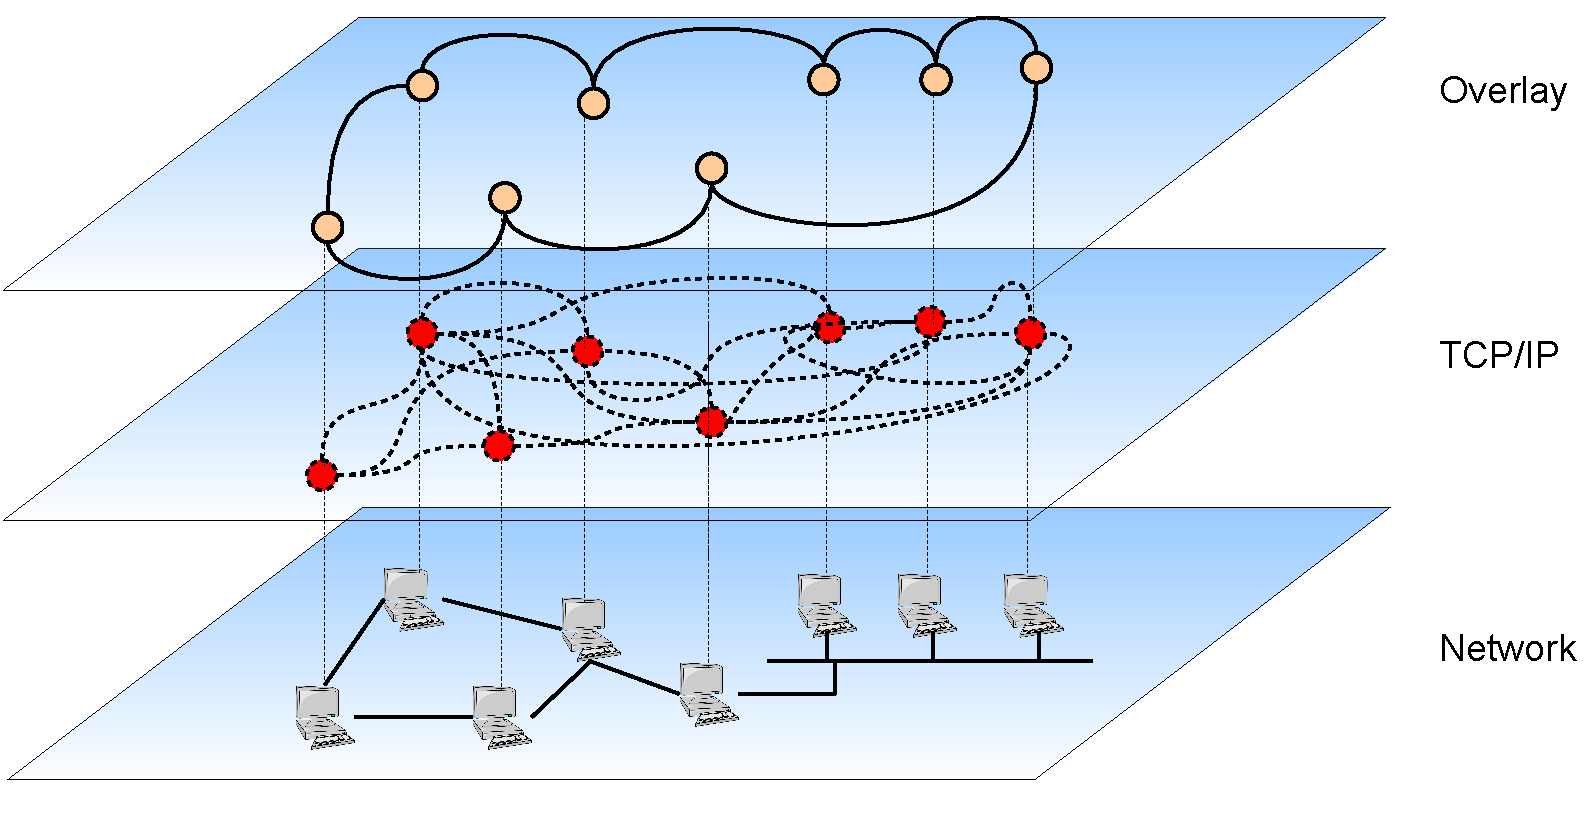
\includegraphics[width=\textwidth]{overlay}
\end{figure}
\end{frame}

\begin{frame}{Overlay networks}

\structure{Virtual edge}\\
\BI
\item TCP connection
\item or simply a pointer to an IP address
\EI

\bigskip
\structure{Overlay maintenance}\\
\BI
\item Periodically ping to make sure neighbor is still alive
\item Or verify liveness while messaging 
\item If neighbor goes down, may want to
establish new edge 
\item New node needs to bootstrap
\EI

\end{frame}

%-------------------------------------------------------------------------

\begin{frame}{Overlay networks}

\begin{columns}
\begin{column}{0.4\textwidth}
\structure{Tremendous design flexibility}\\
\BI
\item Topology
\item Message types
\item Protocols
\item Messaging over TCP or UDP
\EI

\bigskip
\structure{Underlying physical net is transparent to developer}\\
\BI
\item But some overlays exploit proximity
\EI
\end{column}
\begin{column}{0.5\textwidth}
	\begin{figure}
		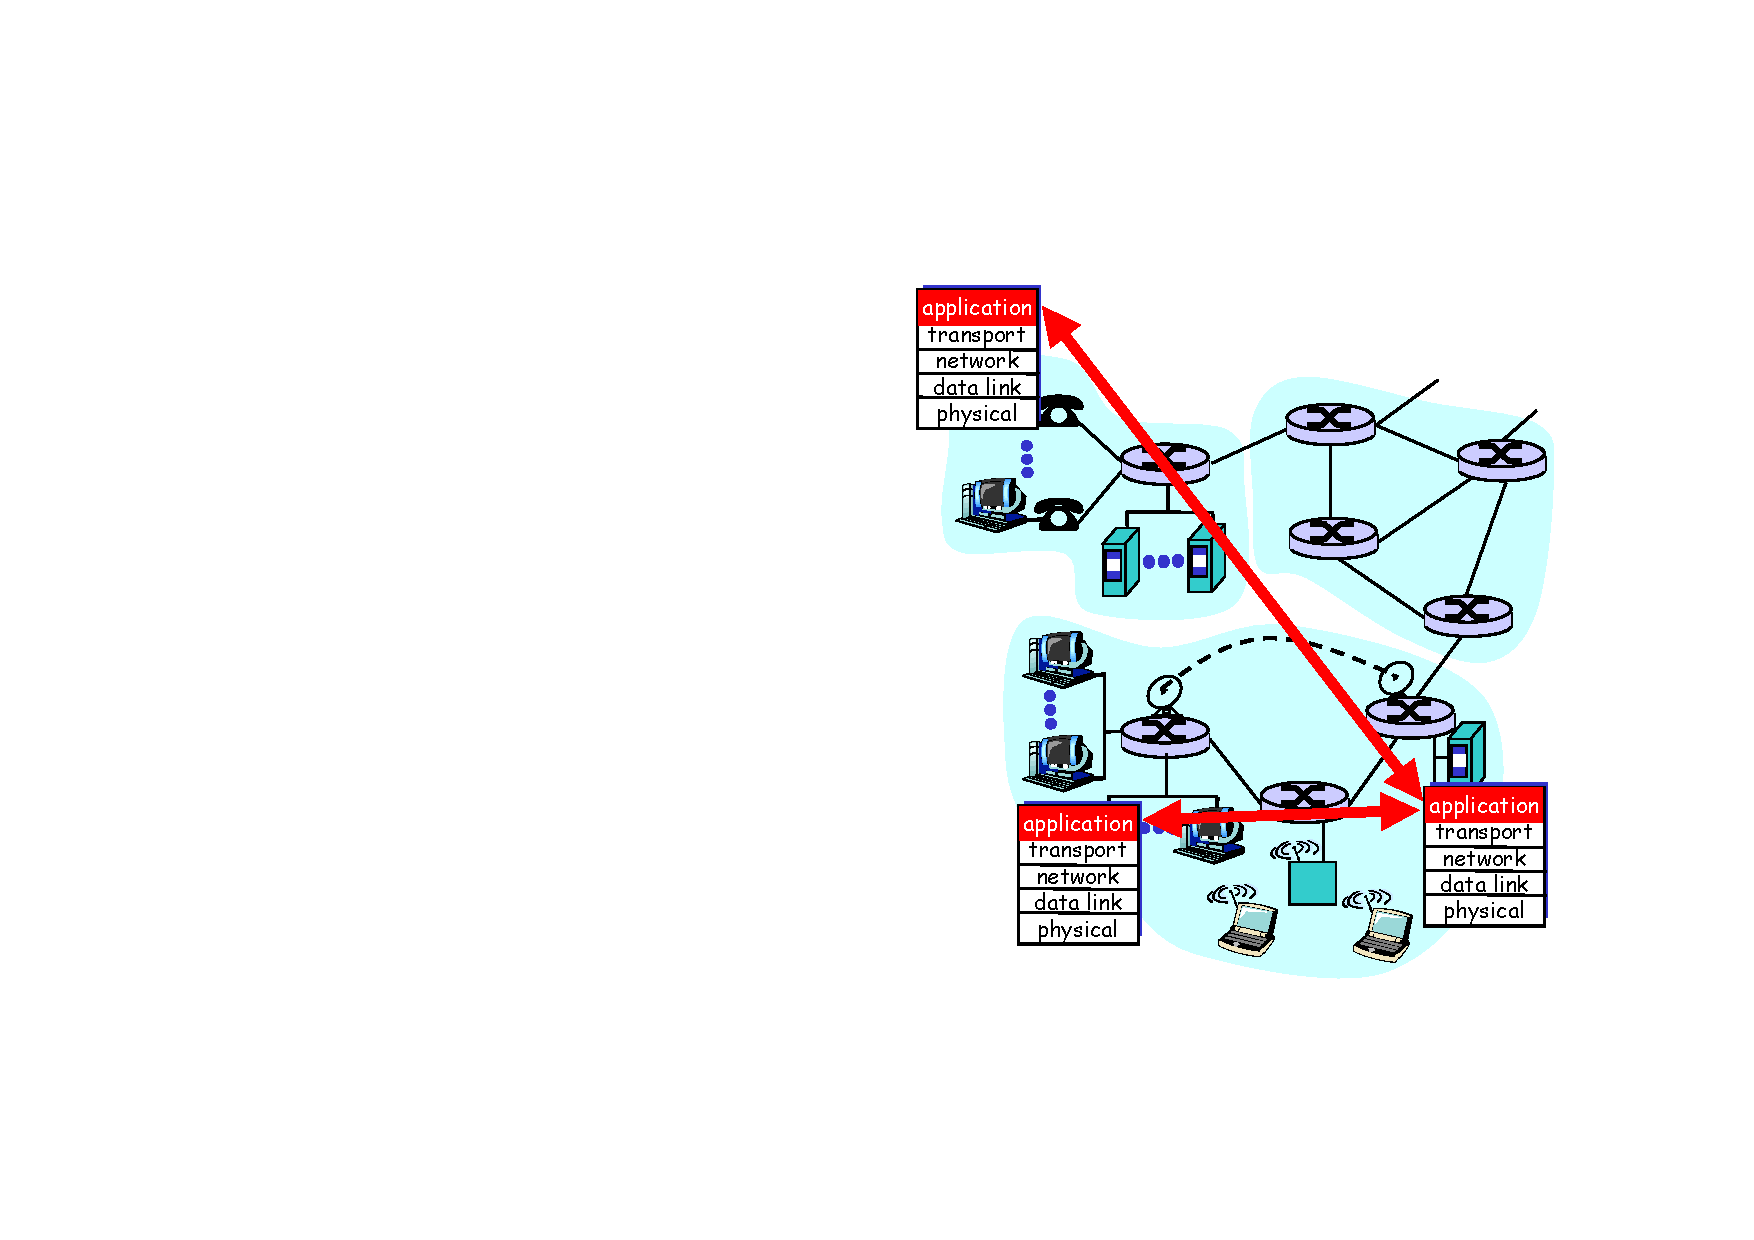
\includegraphics[width=1.0\textwidth]{overlay2.pdf}
	\end{figure}
\end{column}
\end{columns}

\end{frame}

%-------------------------------------------------------------------------

\begin{frame}{Overlay Topology}

\begin{columns}
\begin{column}{0.4\textwidth}
\structure{Unstructured}:
	\BI
	\item No explicit topology
	\item Observed rather than engineered
	\item Example: Gnutella, BitTorrent
	\EI
	
\bigskip
\structure{Structured}:
\BI
\item An explicit “shape” is maintained
\item Examples: Rings, Trees, DHTs
\item Random topologies are “structured” as well
\EI
\end{column}
\begin{column}{0.6\textwidth}
	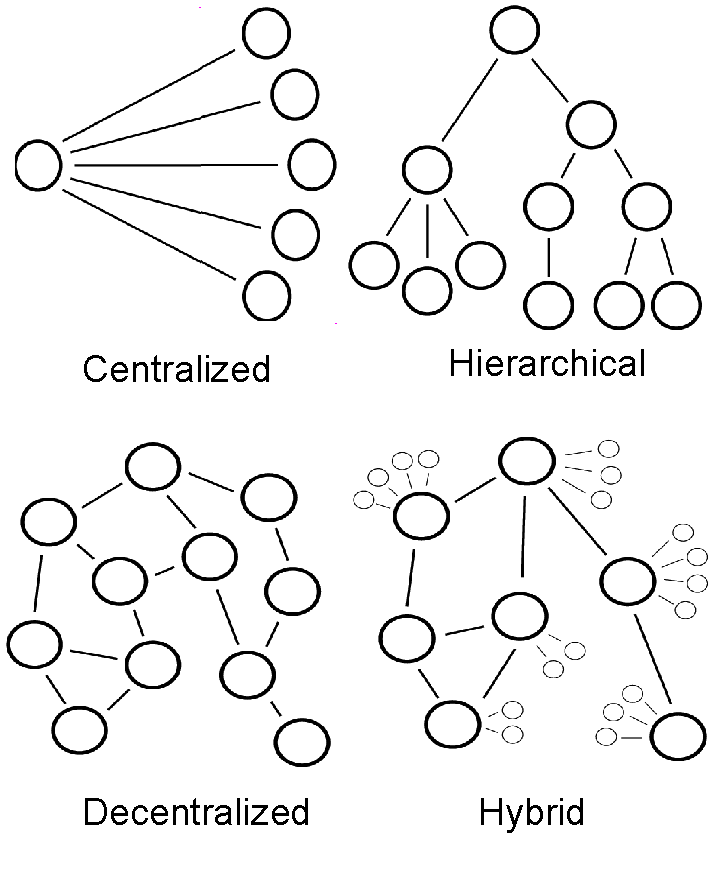
\includegraphics[width=0.9\textwidth]{p2ptypes}
\end{column}
\end{columns}

\end{frame}

%-------------------------------------------------------------------------

\begin{frame}{Criteria for topology selection}
	
	
\BIL
\item Does it simplify location of data?
\item Does it
	\BI
	\item balance the load, if nodes are equal?
	\item exploit heterogeneity, otherwise?
	\EI
\item Is it robust?
	\BI
	\item Can it work if part of it is suddenly removed?
	\item Can it be maintained in spite of churn?
	\EI
\item Has some correspondence with the underlying network topology?
\BI
\item Proximity (latency-based)
\item e.g., Pastry, Kazaa, Skype
\EI
\EIL
\end{frame}


%%%%%%%%%%%%%%%%%%%%%%%%%%%%%%%%%%%%%%%%%%%%%%%%%%%%%%%%%%%%%%%%%%%%%%%%%%
\section{Distributed Hash Tables}

\subsection{Overview}

\begin{frame}{Distributed Hash Table (DHT)}

\structure{A peer-to-peer algorithm that offers an associative \alert{Map} interface}:\\
\BI
\item \alert{$\mathit{put}(\textsc{Key}\ k,\ \textsc{Value}\ v)$}: associate a value $v$ to the key $k$
\item \alert{$\textsc{Value}\ \mathit{get}(\textsc{Key}\ k)$}: returns the value associated to key $k$
\EI

\bigskip
\structure{(Distributed) Hash Tables}:\\
\BI
\item Hash tables map keys to memory locations
\item Distributed hash tables map keys to nodes
\EI

\bigskip
\structure{Organization}:\\
\BI
\item Each node is responsible for a portion of the key space
\item Messages are routed between nodes to reach responsible nodes
\item Replication used to tolerate failures
\EI

\end{frame}

\begin{frame}{Routing in DHTs}

\begin{figure}
	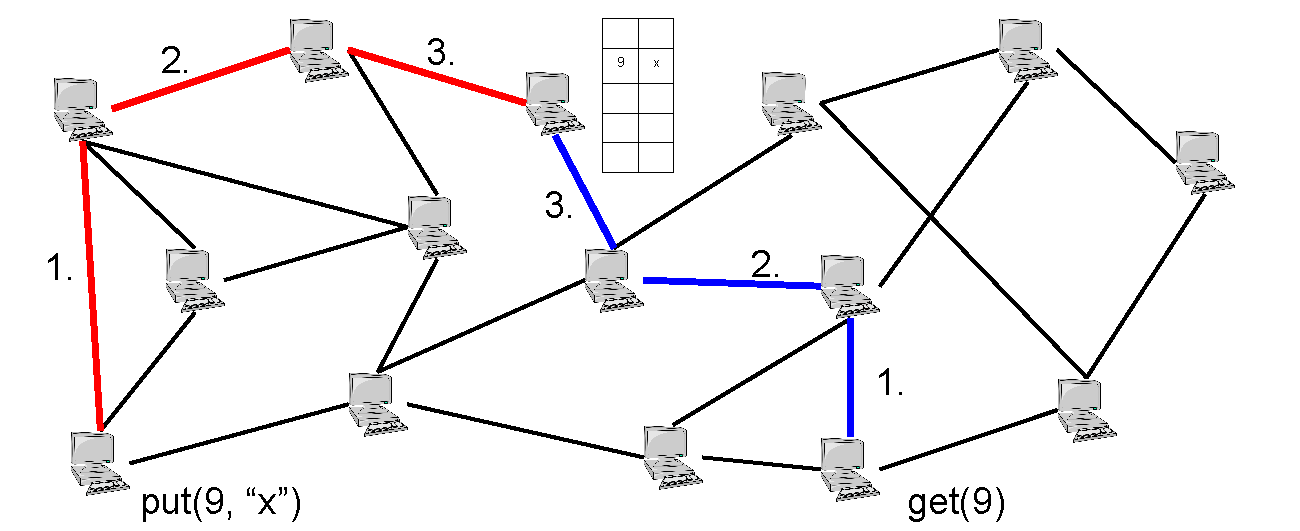
\includegraphics[width=\textwidth]{dht-routing}
\end{figure}

\end{frame}

%-------------------------------------------------------------------------
\begin{frame}{DHT Implementations}
	
\BIL
\item The founders (2001):
	\BI
	\item \alert{Chord}
	\item \alert{CAN}
	\item Pastry
	\item Tapestry
	\EI
\item The ones which are actually used:
	\BI
	\item \alert{Kademlia} and its derivatives (up to 4M nodes!)
		\BI
		\item BitTorrent
		\item Kad (eMule)
		\item The Storm Botnet
		\EI
	\item \alert{Cassandra} DHT
		\BI
		\item Part of Apache Cassandra
		\item Initially developed at Facebook
		\EI
	\EI
\item The ones which are actually used, but we don't know much about:
\BI
\item Microsoft DHT based on Pastry
\item Amazon's Dynamo key-value store
\EI
\EIL
\end{frame}

%-------------------------------------------------------------------------
\begin{frame}{Step 1: From Keys and Nodes to IDs}

\BIL
\item Keys and nodes are represented by \alert{identifiers} taken from an \alert{ID space} 
\BI
\item Key identifiers: computed through an \alert{hash function} (e.g., SHA-1)
  \BI
  \item e.g., $\ID(k) = \mathit{SHA}1(k)$
  \EI
\item Node identifiers: randomly assigned or computed through an hash function
  \BI
  \item e.g., $\ID(n) =\mathit{SHA}1(\textrm{IP address of $n$})$
  \EI
\EI
\EIL

\bigskip
\structure{Why?}\\
\BIL
\item Very low probability that two nodes have exactly the same ID
\item Nodes and keys are mapped in the same space
\EIL

\end{frame}

%-------------------------------------------------------------------------
\begin{frame}{Step 2: Partition the ID space}

\BIL
\item Each node in the DHT stores some $k,v$ pairs
\item Partition the ID space in zones, depending on the node IDs:
\item A pair $(k,v)$ is stored at the node $n$ such that (examples):
\BI
\item its identifier $\ID(n)$ is the closest to $\ID(k)$;
\item its identifier $\ID(n)$ is the largest node id smaller than $\ID(k)$
\EI
\EIL

\begin{figure}
	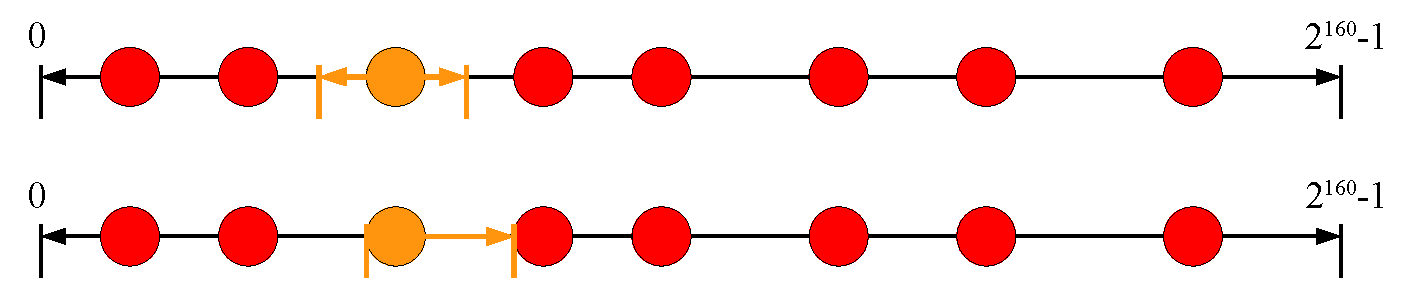
\includegraphics[width=\textwidth]{dht-partition}
\end{figure}

\end{frame}

%-------------------------------------------------------------------------
\begin{frame}{Step 2: Build overlay network}

Each node has two sets of neighbors:
\BIL
\item Immediate neighbors in the key space (leafs)
  \BI
  \item Guarantee correctness, avoid partitions
  \item If we had only them, linear routing time
  \EI
\item Long-range neighbors
  \BI
  \item Allow sub-linear routing
  \item If we had only them, connectivity problems
  \EI
\EIL

\begin{figure}
	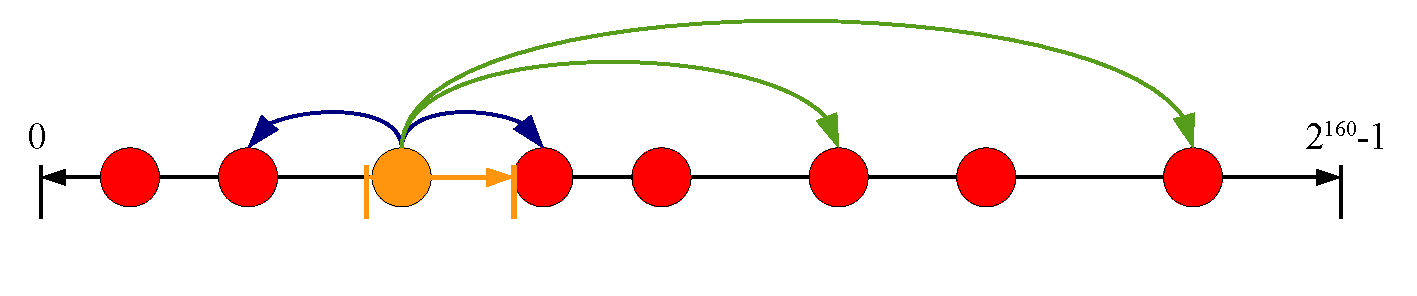
\includegraphics[width=\textwidth]{dht-overlay}
\end{figure}

\end{frame}

%-------------------------------------------------------------------------
\begin{frame}{Step 3: Route puts/gets through the overlay}

\BI
\item \alert{Recursive routing}: the initiator starts the process, contacted
  nodes forward the message	
\item \alert{Iterative routing}: the initiator personally contact the nodes at each
  routing step
\EI

\begin{figure}
	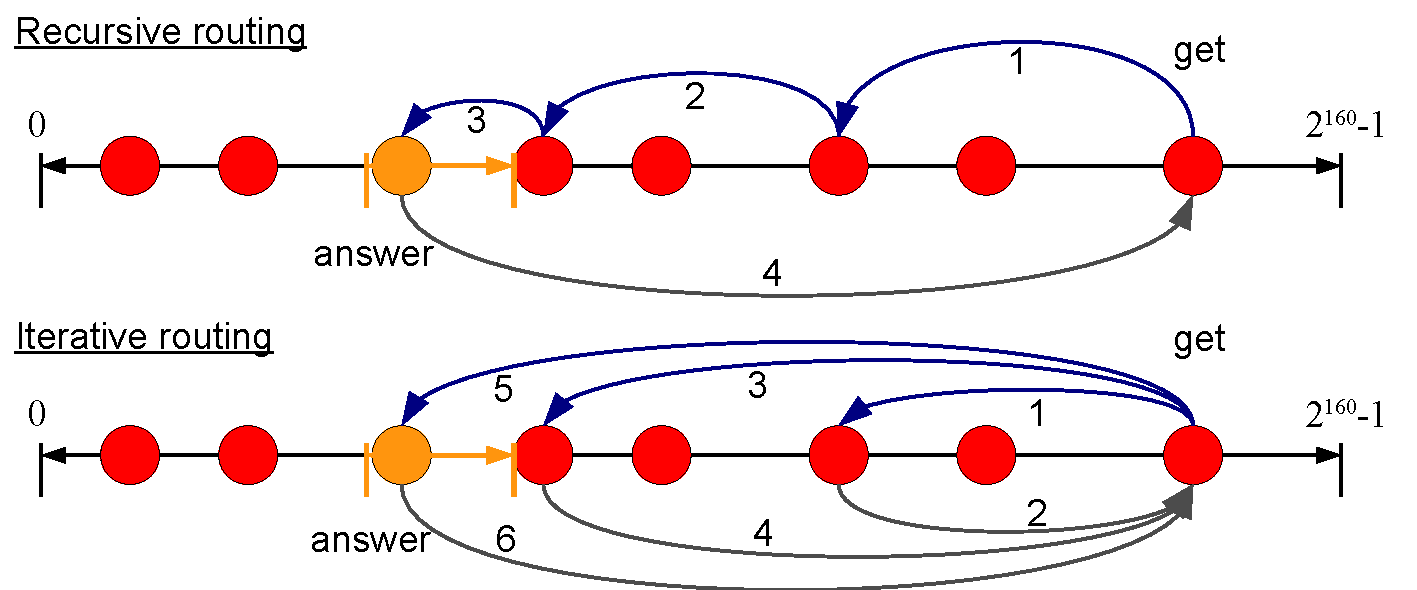
\includegraphics[width=\textwidth]{dht-route}
\end{figure}

\end{frame}

%-------------------------------------------------------------------------
\begin{frame}{Routing around failures (1)}

\BI
\item Under churn, neighbors may have failed
\item To detect failures, acknowledge each hop (recursive routing)
\EI

\begin{figure}
	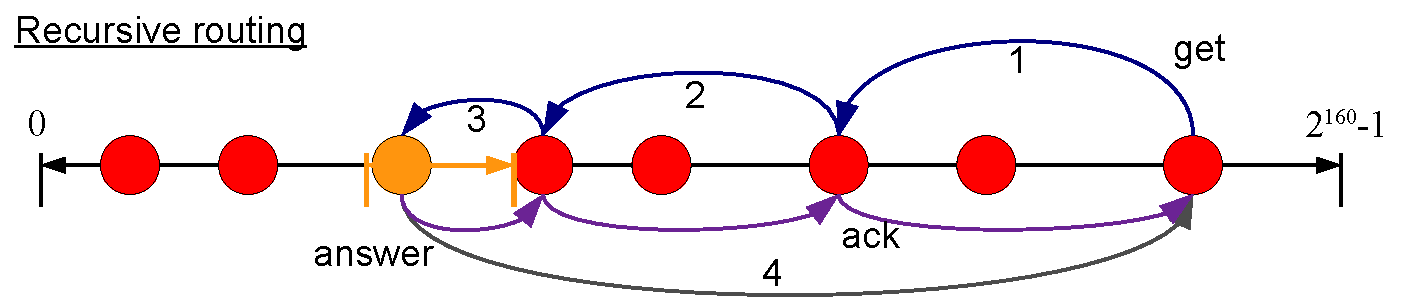
\includegraphics[width=\textwidth]{dht-route-failure}
\end{figure}

\end{frame}

%-------------------------------------------------------------------------
\begin{frame}{Routing around failures (2)}

\BI
\item If we don't receive ack or response, resend through a different neighbor
\EI

\begin{figure}
	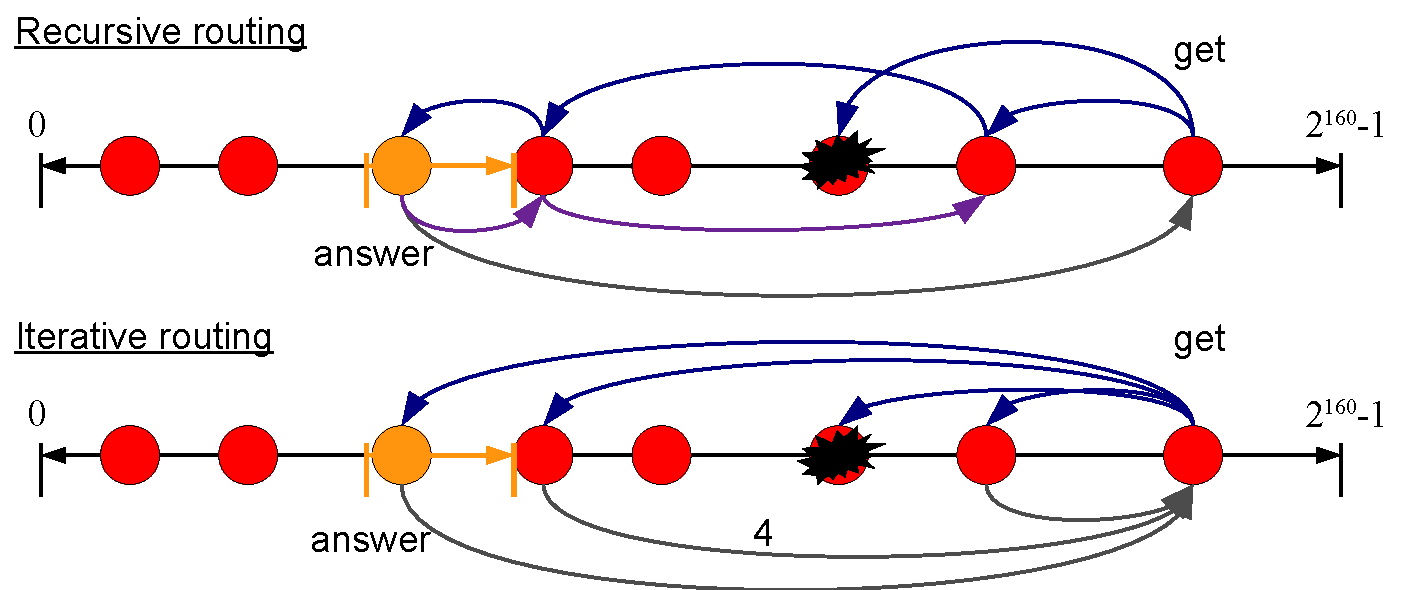
\includegraphics[width=\textwidth]{dht-route-failure2}
\end{figure}

\end{frame}

%-------------------------------------------------------------------------
\begin{frame}{Routing around failures (3)}

\BIL
\item Must compute timeouts carefully
\BI
\item If too long, increase put/get latency
\item If too short, get message explosion
\EI
\item Parallel sending could be a design decision -- see Kademlia
\EIL

\begin{figure}
	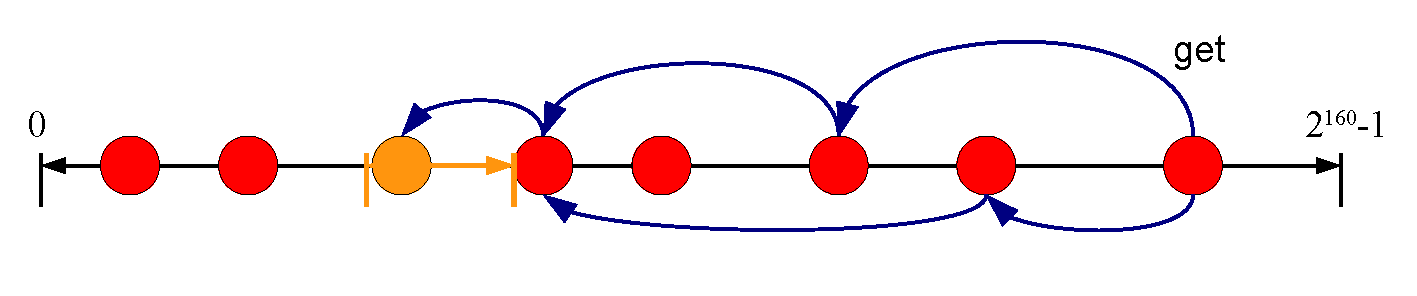
\includegraphics[width=\textwidth]{dht-route-failure3}
\end{figure}

\end{frame}

%-------------------------------------------------------------------------
\begin{frame}{Computing good timeouts}
	
\BIL
\item Use TCP-style timers
	\BI
	\item Keep past history of latencies
	\item Use this to compute timeouts for new requests
	\EI
\item Works fine for recursive lookups
	\BI
	\item Only talk to neighbors, so history small, current
	\EI
\item In iterative lookups, source leads the  entire lookup process
	\BI
	\item Must potentially have good timeout for any node
	\EI
\EIL

\end{frame}

%-------------------------------------------------------------------------
\begin{frame}{Recovering from failures}

\BIL
\item Can't route around failures forever 
	\BI
	\item Will eventually run out of neighbors
	\EI
\item Must also find new nodes as they join
	\BI
	\item Especially important if they're our immediate predecessors or successors
	\EI
\EIL

\begin{figure}
	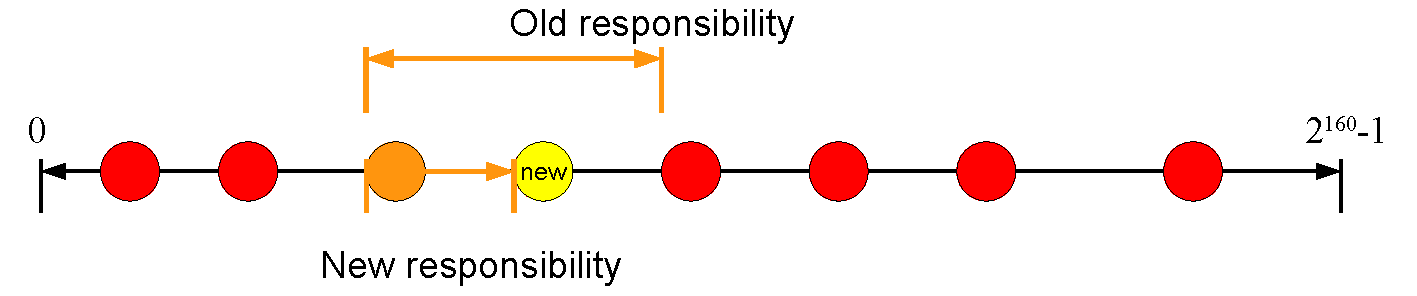
\includegraphics[width=\textwidth]{dht-recovery}
\end{figure}

\end{frame}

\begin{frame}{Recovery from failures}

\BIL
\item \alert{Reactive recovery}
\BI
\item When a node stops sending acknowledgments, notify other neighbors of potential replacements
\EI
\item \alert{Proactive recovery}
\BI
\item Periodically, each node sends its neighbor list to each of its neighbors
\EI
\EIL

\begin{figure}
	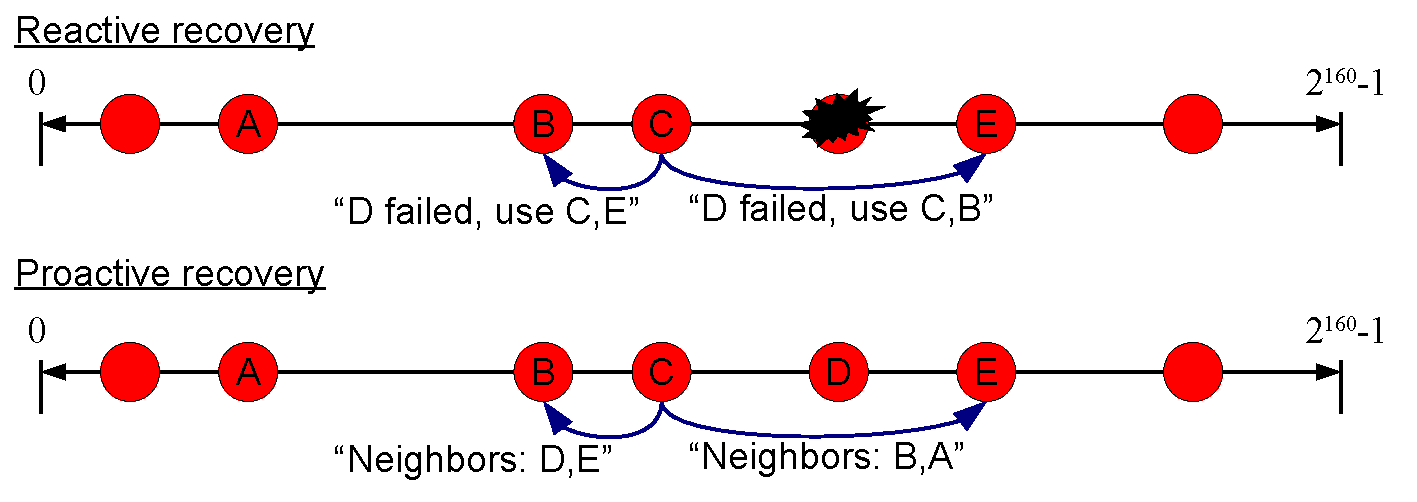
\includegraphics[width=\textwidth]{dht-repair}
\end{figure}

\end{frame}

\subsection{Chord}

%-------------------------------------------------------------------------
\begin{frame}{Chord}

\begin{columns}
\begin{column}{0.72\textwidth}
\BI
\item ID space: uni-dimensional ring in $[0, 2^{m}-1]$ ($m=160$)
\item Routing table size: $O(\log n)$
\item Routing time: $O(\log n)$	
\EI
\end{column}
\begin{column}{0.28\textwidth}
\begin{figure}
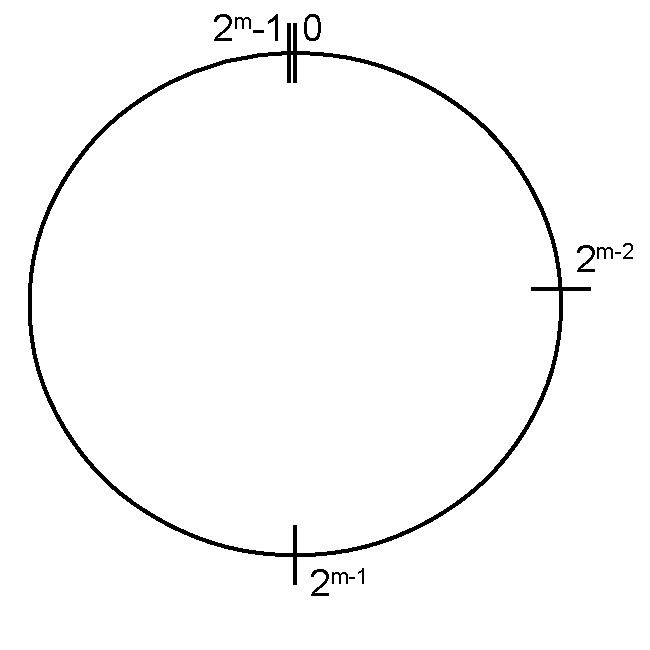
\includegraphics[width=1.0\textwidth]{chord-example1}
\end{figure}
\end{column}
\end{columns}

\begin{Bib}
{\scriptsize
\bibentry{chord}
}\end{Bib}
	
\end{frame}

%-------------------------------------------------------------------------
\begin{frame}{Identifier mapping}

\begin{columns}
\begin{column}{0.4\textwidth}
\structure{Example}:
\BI
\item Node  $8$ maps $[5,8]$
\item Node $15$ maps $[9,15]$
\item Node $20$ maps $[16, 20]$
\item \ldots
\item Node $4$ maps $[59, 4]$
\EI

\bigskip
\BI
\item Random ID assignment
\item Each node maintains a pointer to its successor
\EI
\end{column}
\begin{column}{0.6\textwidth}
\begin{figure}
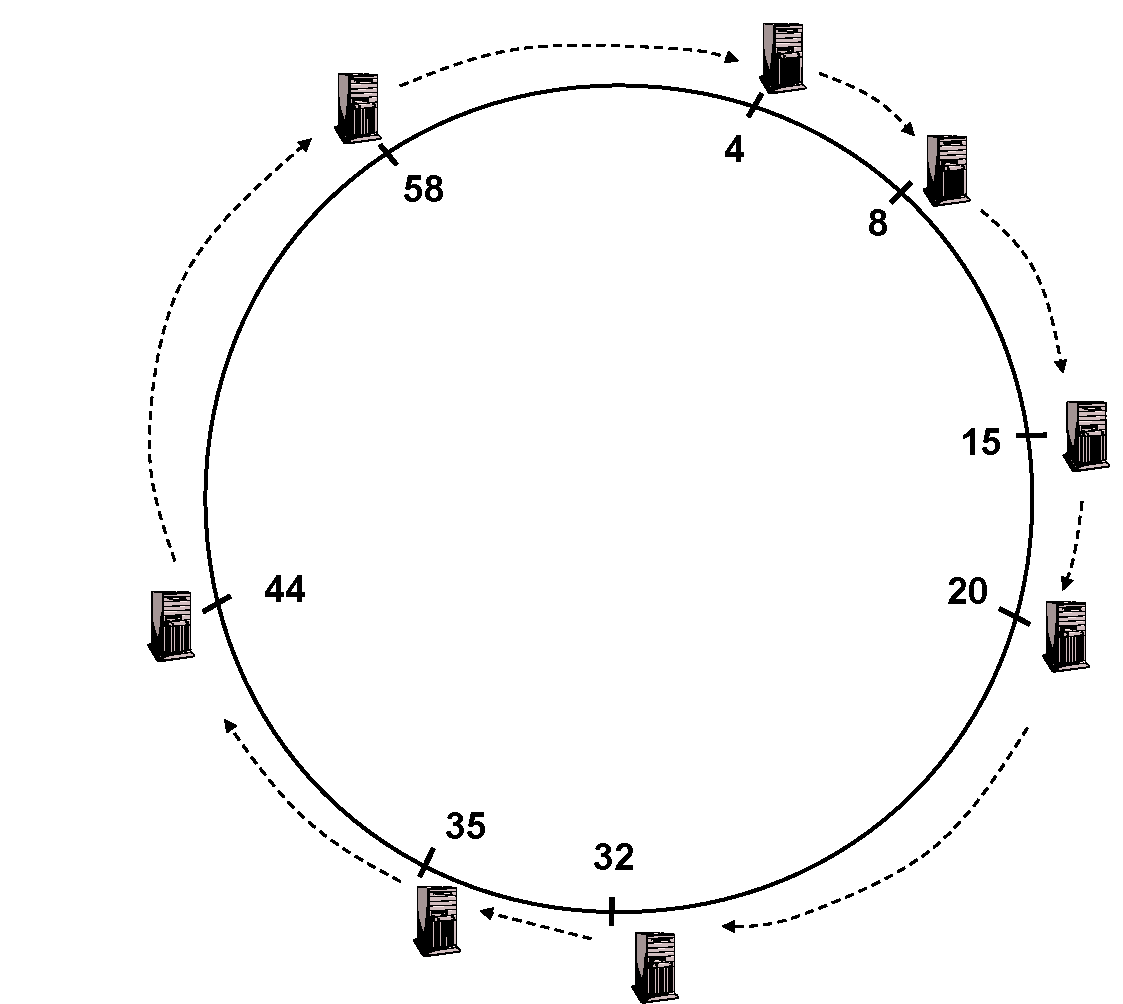
\includegraphics[width=1.0\textwidth]{chord-example2}
\end{figure}
\end{column}
\end{columns}

\end{frame}

%-------------------------------------------------------------------------
\begin{frame}{Join procedure (1)}

\begin{columns}
\begin{column}{0.4\textwidth}
\structure{Example}:
\BI
\item Node with $\mathit{id}=50$ joins the ring
\item Node 50 needs to know at least one node already in the system
\item Assume known node is 15		
\EI

\end{column}
\begin{column}{0.6\textwidth}
\begin{figure}
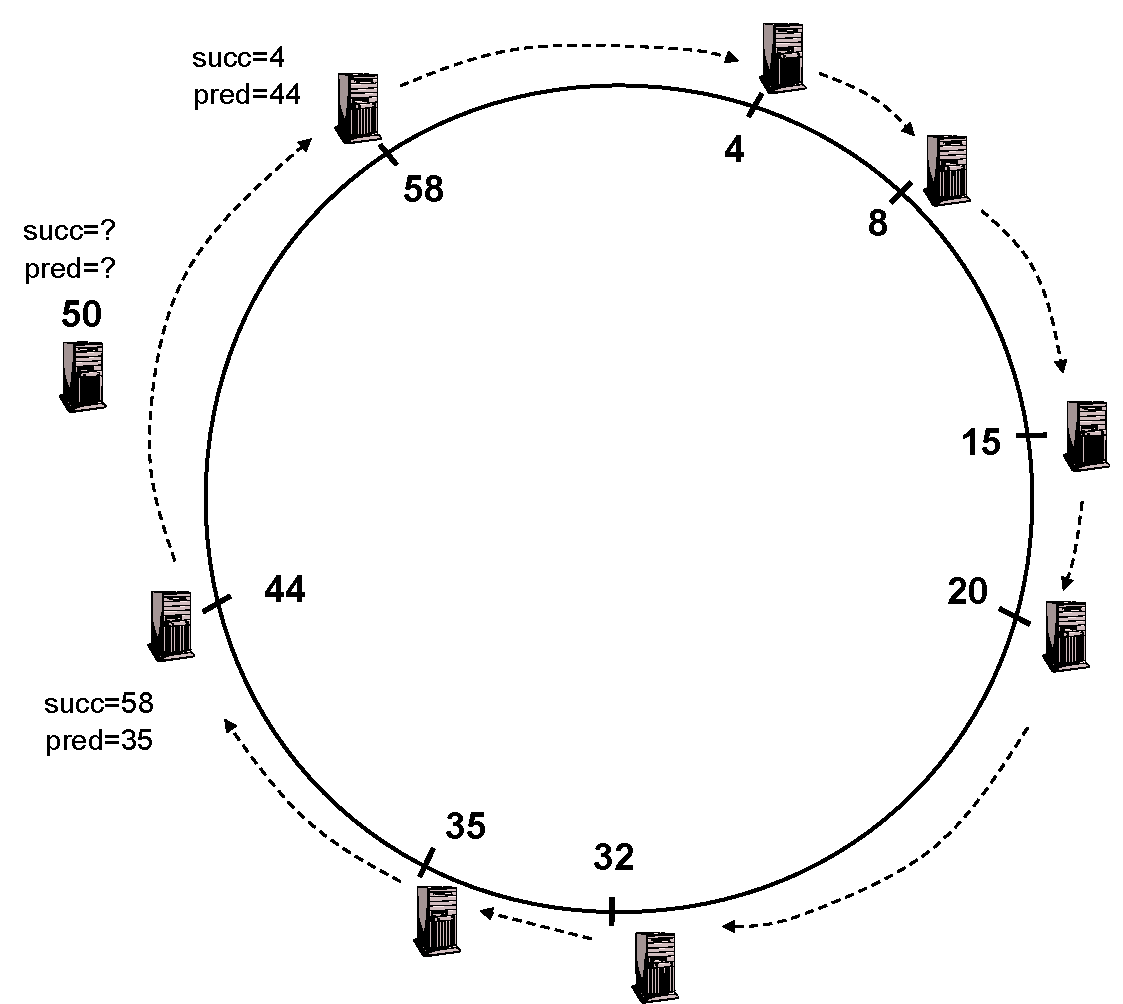
\includegraphics[width=1.0\textwidth]{chord-example3}
\end{figure}
\end{column}
\end{columns}

\end{frame}

%-------------------------------------------------------------------------
\begin{frame}{Join procedure (2)}

\begin{columns}
\begin{column}{0.4\textwidth}
\structure{Example}:
\BI
\item Node $50$: send $\langle \textsc{join}, 50 \rangle$ to node $15$ 
\item Message is routed to node $44$
\item Node $44$: returns node $58$ 
\item Node $50$: updates its successor to $58$
\EI

\end{column}
\begin{column}{0.6\textwidth}
\begin{figure}
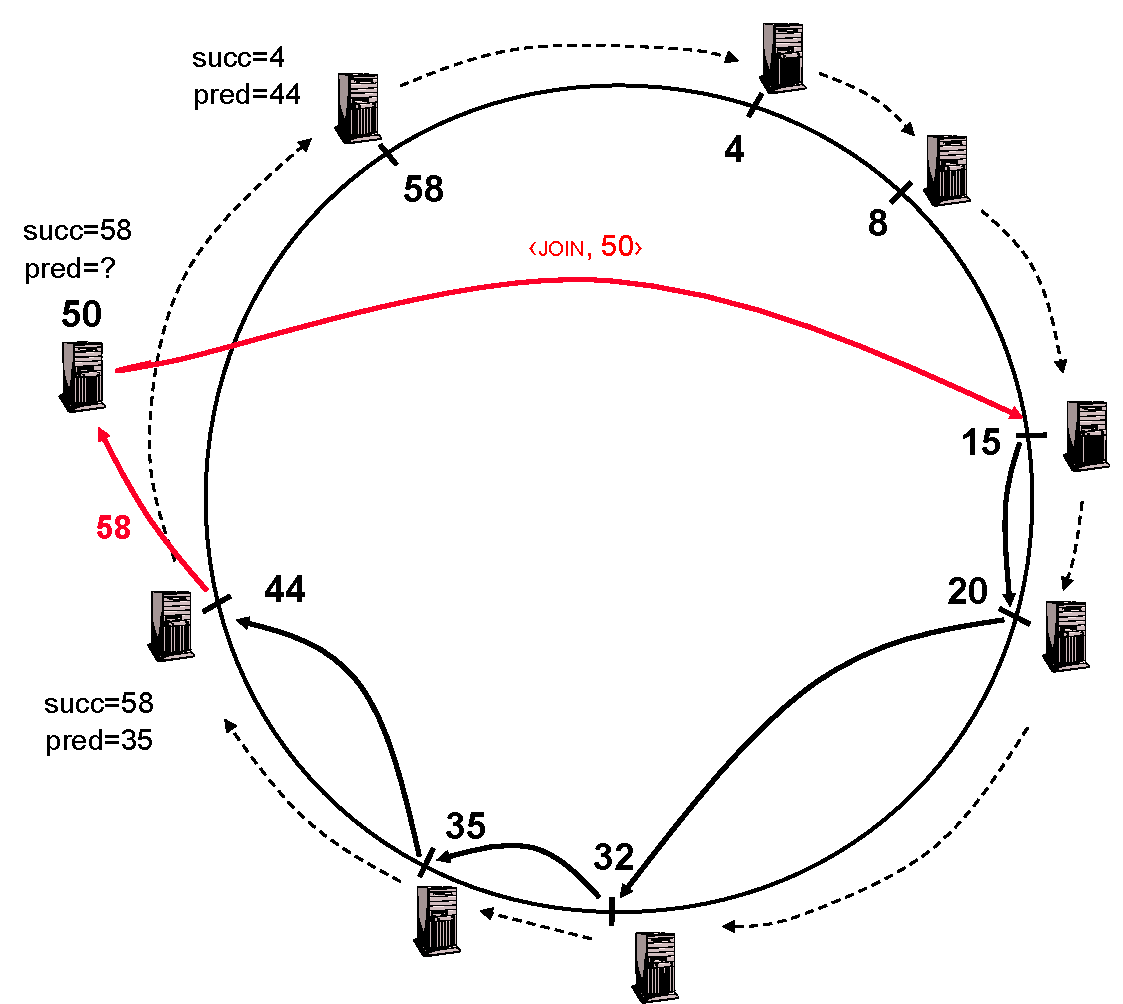
\includegraphics[width=1.0\textwidth]{chord-example4}
\end{figure}
\end{column}
\end{columns}

\end{frame}

%-------------------------------------------------------------------------
\begin{frame}{Stabilization}

\BIL
\item Periodically, each node $A$:
\BI
\item sends a $\langle \textsc{stabilize} \rangle$ message to its successor $B$
\EI
\item Upon receiving $\langle \textsc{stabilize} \rangle$ message from $A$, node $B$:
\BI
\item returns its predecessor $B'=\mathit{pred}(B)$ to $A$ by sending a $\langle \textsc{notify}, B' \rangle$ message
\item updates its predecessor to $A$, if $A$ is between $B'$ and $B$
\EI
\item Upon receiving $\langle \textsc{notify}, B' \rangle$ message from $B$, node $A$:
\BI
\item updates its successor to $B'$, if $B'$ is between $A$ and $B$
\EI
\EIL

\end{frame}

%-------------------------------------------------------------------------
\begin{frame}{Join procedure (4)}

\begin{columns}
\begin{column}{0.4\textwidth}
\structure{Example}:
\BI
\item Node $50$: send $\langle \textsc{stabilize} \rangle$ to node $58$ 
\item Node $58$: update predecessor to $50$  
\item Node $58$: send $\langle \textsc{notify}, 50 \rangle$ back
\EI

\end{column}
\begin{column}{0.6\textwidth}
\begin{figure}
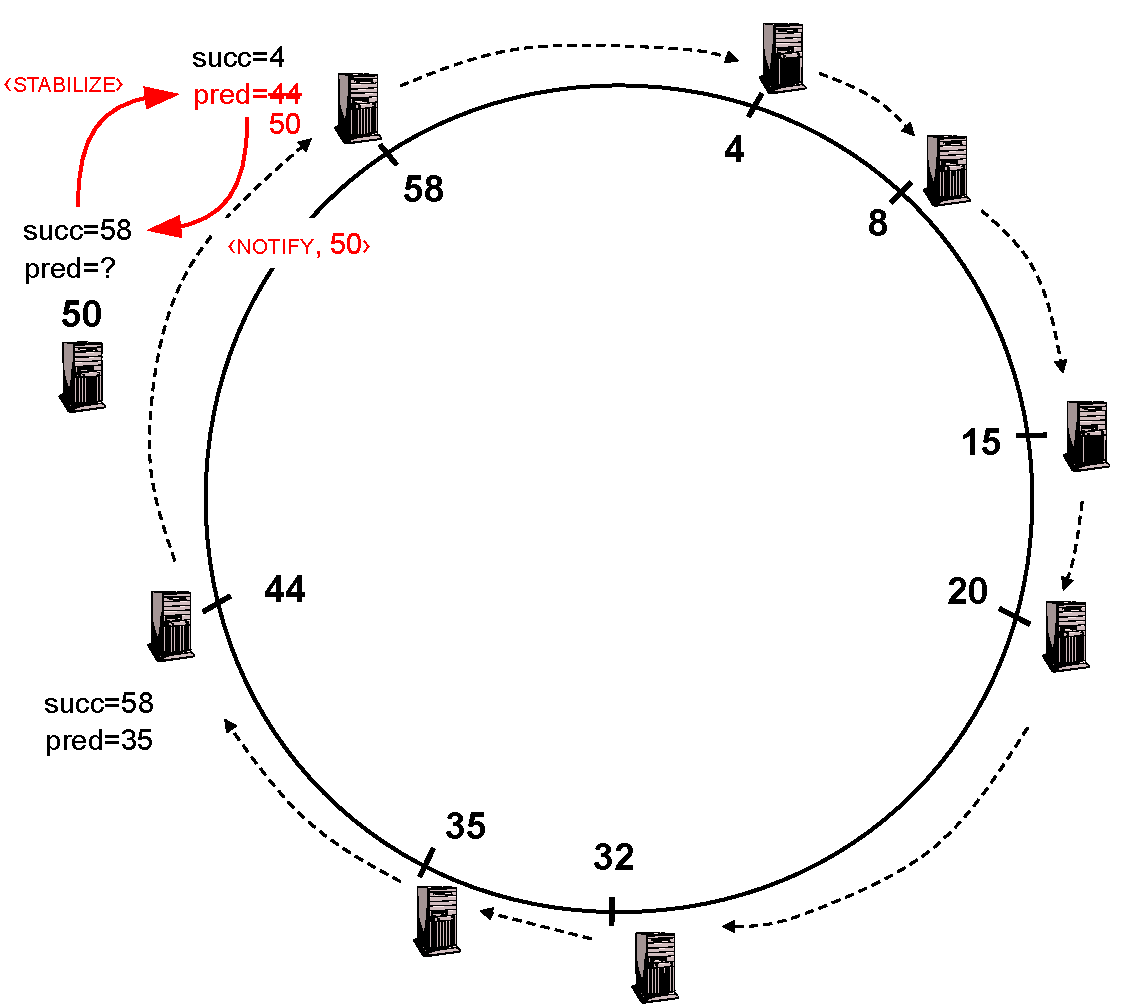
\includegraphics[width=1.0\textwidth]{chord-example5}
\end{figure}
\end{column}
\end{columns}

\end{frame}

%-------------------------------------------------------------------------
\begin{frame}{Join procedure (5)}

\begin{columns}
\begin{column}{0.4\textwidth}
\structure{Example}:
\BI
\item Node $44$: send $\langle \textsc{stabilize} \rangle$ to its successor node $58$ 
\item Node $58$: replies with  $\langle \textsc{notify}, 50 \rangle$ 
\item Node $44$: updates it successor to $50$
\EI

\end{column}
\begin{column}{0.6\textwidth}
\begin{figure}
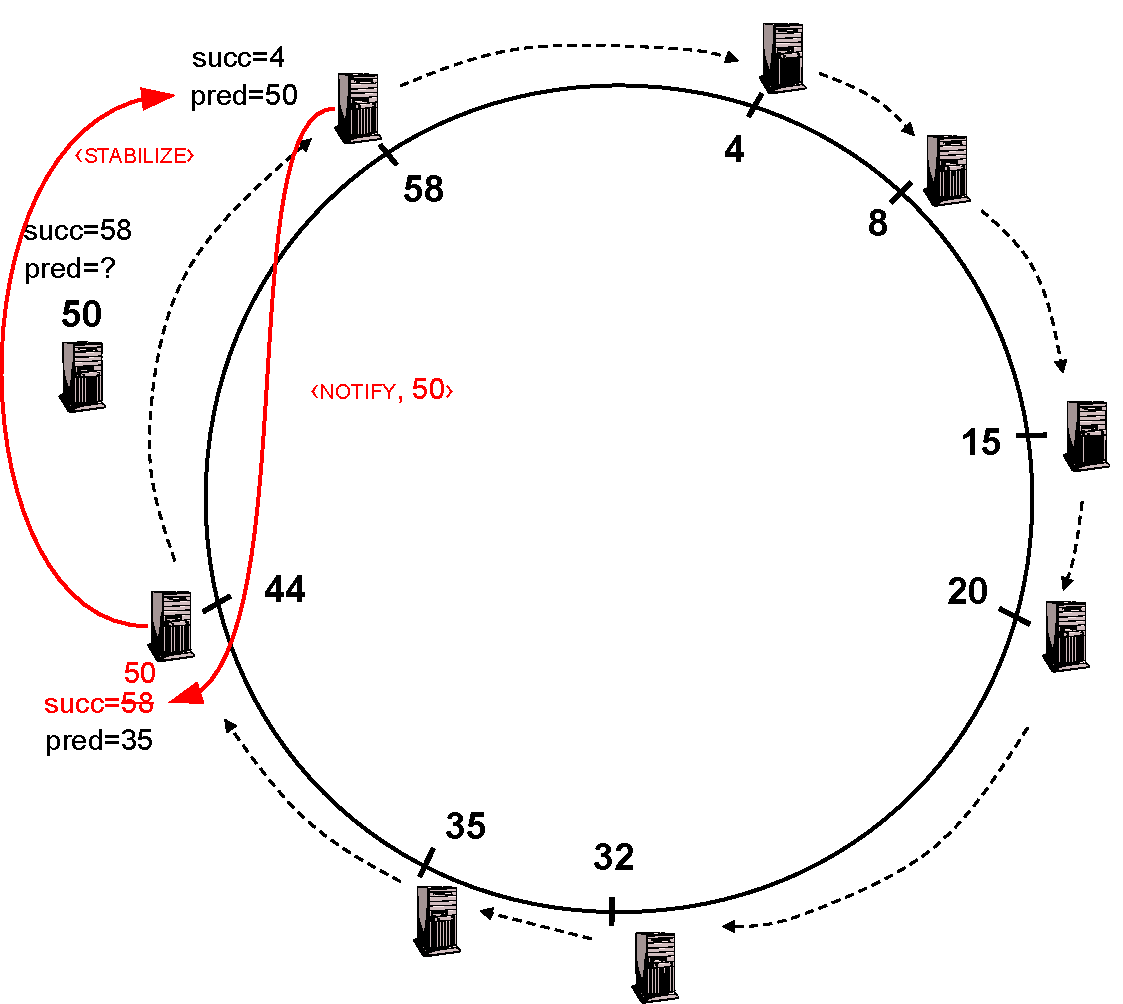
\includegraphics[width=1.0\textwidth]{chord-example6}
\end{figure}
\end{column}
\end{columns}

\end{frame}


%-------------------------------------------------------------------------
\begin{frame}{Join procedure (6)}

\begin{columns}
\begin{column}{0.4\textwidth}
\structure{Example}:
\BI
\item Node $44$: send $\langle \textsc{stabilize} \rangle$ to its new successor, node $50$ 
\item Node $50$: updates it predecessor to $44$
\EI
This completes the joining operation!

\end{column}
\begin{column}{0.6\textwidth}
\begin{figure}
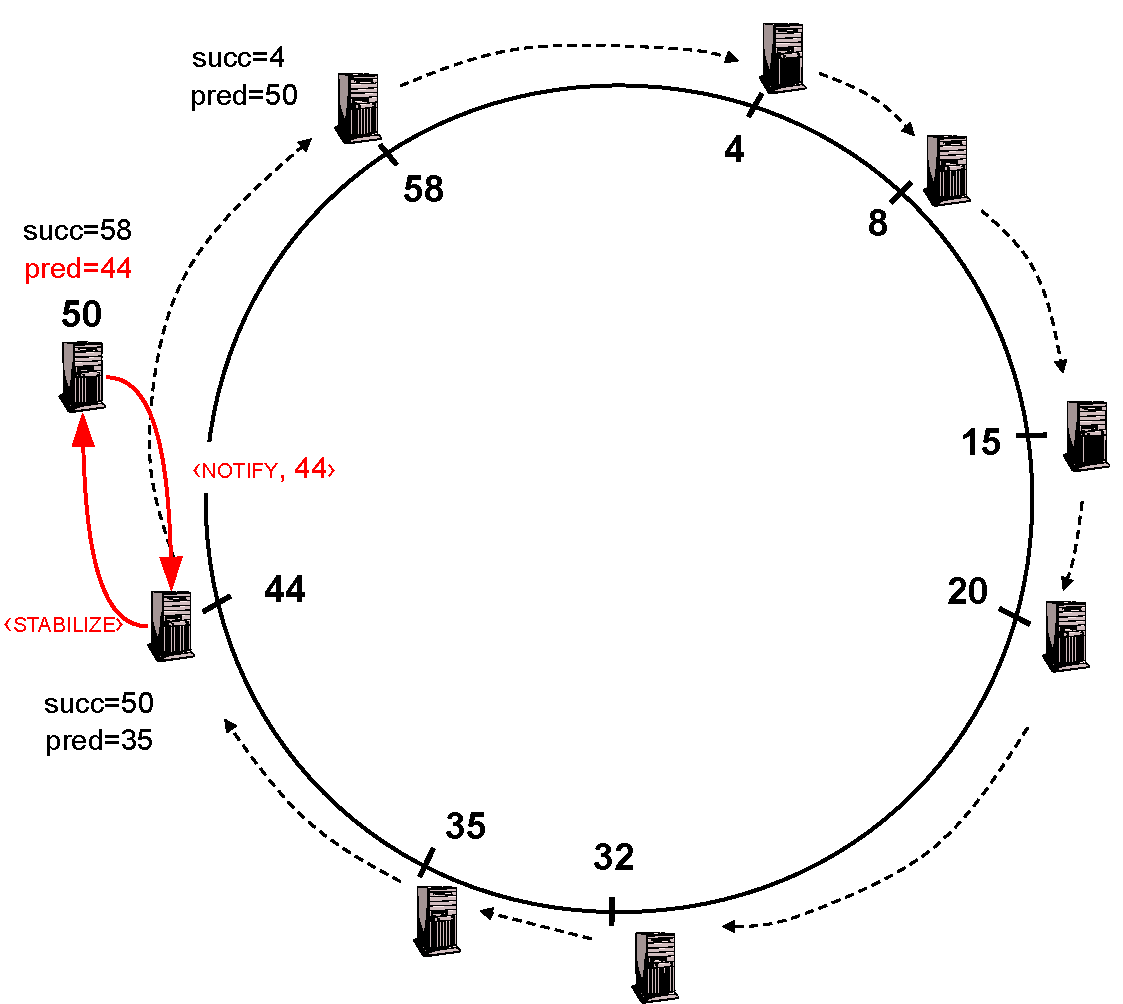
\includegraphics[width=1.0\textwidth]{chord-example7}
\end{figure}
\end{column}
\end{columns}

\end{frame}

%-------------------------------------------------------------------------
\begin{frame}{Achieving efficiency}

\BIL
\item Chord requires each node to keep a \alert{finger table} containing 
up to $m$ entries
\item The $i$-th entry ($0 \leq i \leq m-1$) of node $n$ will contain the 
address of the successor of $(n + 2^{i}) \bmod 2^m$
\item Fingers are used in routing to reduce the number of hops to $O(\log N)$
\EIL
\end{frame}

%-------------------------------------------------------------------------
\begin{frame}{Achieving efficiency}
	
\begin{figure}
	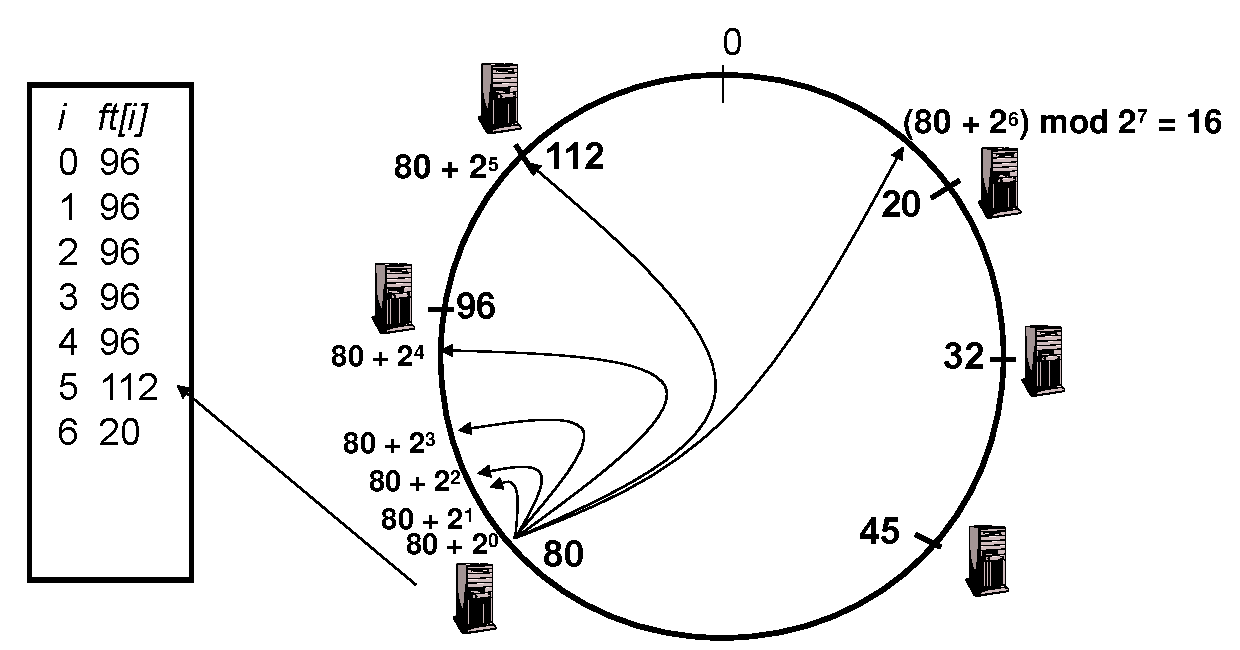
\includegraphics[width=\textwidth]{fingers}
\end{figure}	
	
\end{frame}

%-------------------------------------------------------------------------
\begin{frame}{Achieving robustness}
	
\BI
\item To improve robustness, each node maintains $k > 1$ immediate successors instead of only one
\item In the $\langle \textsc{notify} \rangle$ message, node $A$ can send its $k-1$ successors to its predecessor $B$
\item Upon receiving the $\langle \textsc{notify} \rangle$ message, $B$ can update its successor list 
by concatenating the successor list received from $A$ with $A$ itself
\EI
\end{frame}

%-------------------------------------------------------------------------
\begin{frame}{Optimizations}
	
\BIL
\item \alert{Reduce latency}
	\BI
	\item Choose finger that reduces expected time to reach destination
	\item Choose the closest node from range $[n+2^{i-1},n+2^i)$ as successor
	\EI
\item \alert{Accommodate heterogeneous systems}
	\BI
	\item Multiple virtual nodes per physical node
	\EI
\EIL

\end{frame}

%%%%%%%%%%%%%%%%%%%%%%%%%%%%%%%%%%%%%%%%%%%%%%%%%%%%%%%%%%%%%%%%%%%%%%%%%%

\subsection{CAN}

%-------------------------------------------------------------------------
\begin{frame}{CAN}

\begin{columns}
\begin{column}{0.5\textwidth}
\BI
\item Associate to each node and item a unique ID in an $d$-dimensional Cartesian space on a $d$-torus
\item Routing table size is \alert{constant: $O(d)$}
\item Guarantees that a key is found in at most $d \cdot n^{1/d}$ steps, where $n$ is the total number of nodes	
\EI
\end{column}
\begin{column}{0.5\textwidth}
\begin{figure}
	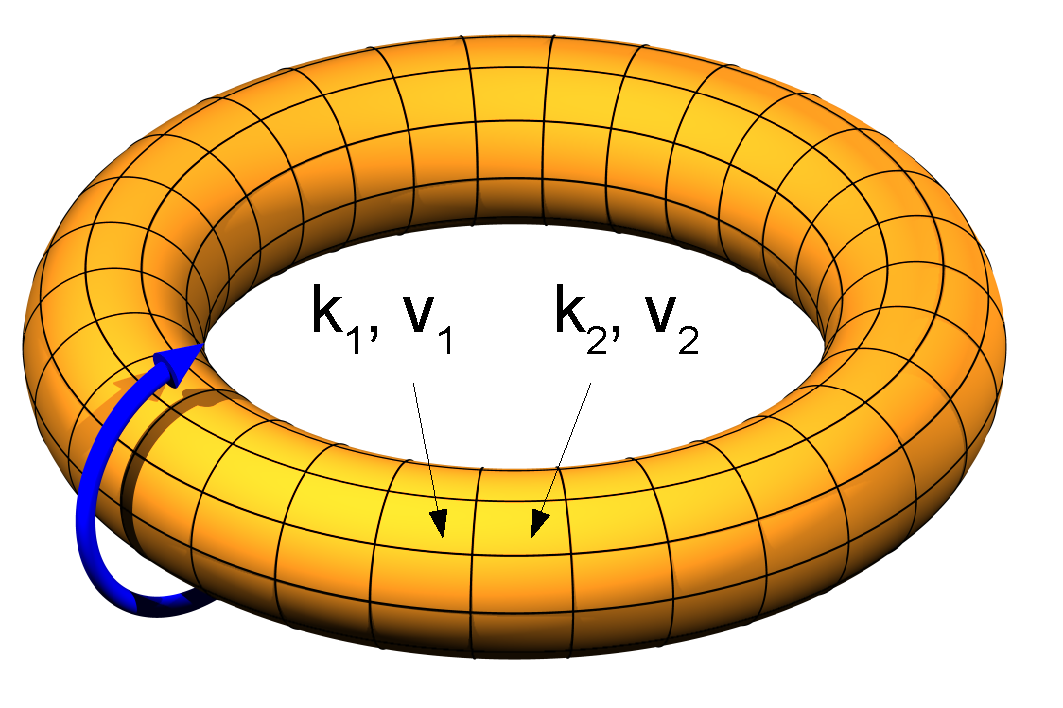
\includegraphics[width=0.8\textwidth]{can-torus}
	\caption{A $2$-torus}
\end{figure}
\end{column}
\end{columns}

\begin{Bib}
{\scriptsize
	\bibentry{can}
}
\end{Bib}

\end{frame}

%-------------------------------------------------------------------------
\begin{frame}{Example: 2-dimensional space}

\begin{columns}
\begin{column}{0.5\textwidth}
\BIL
\item Space divided between nodes
\item All nodes cover the entire space
\item Each node covers either a square or a rectangular area of ratios $1:2$ or $2:1$
\EIL

\smallskip
\structure{Example}:\\
\BI
	\item Node $n_1:(1, 2)$ -- first node that joins -- cover the entire space
\EI
\end{column}
\begin{column}{0.5\textwidth}
\begin{figure}
	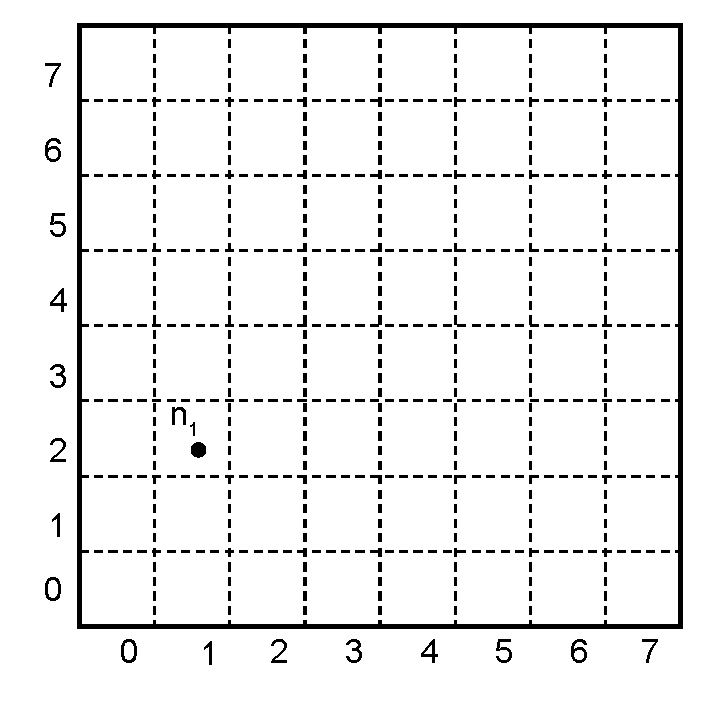
\includegraphics[width=1.0\textwidth]{can1}
\end{figure}
\end{column}
\end{columns}
		
\end{frame}	


%-------------------------------------------------------------------------
\begin{frame}{Example: 2-dimensional space}

\begin{columns}
\begin{column}{0.5\textwidth}
\structure{Example}:\\
\BI
\item Node $n_2:(4, 2)$ joins: space is divided between $n_1$ and $n_2$
\EI
\end{column}
\begin{column}{0.5\textwidth}
\begin{figure}
	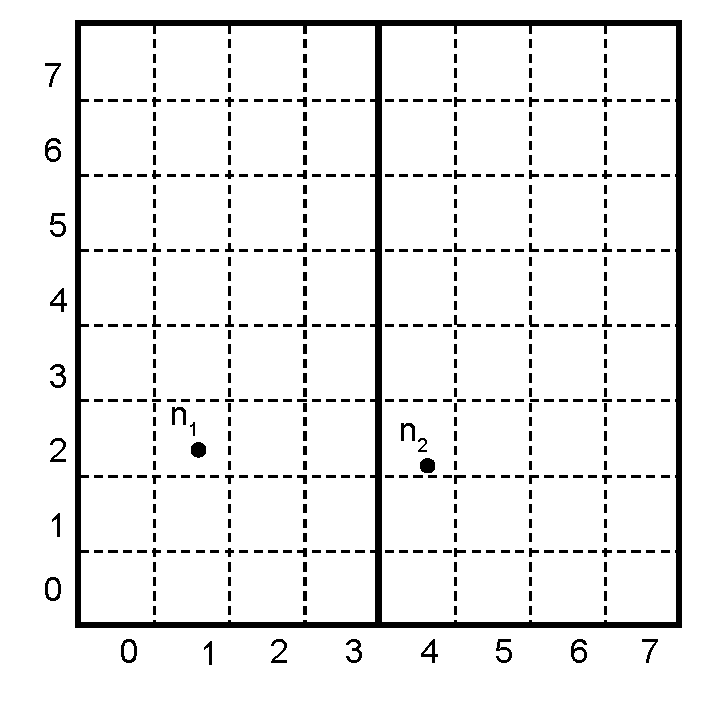
\includegraphics[width=1.0\textwidth]{can2}
\end{figure}
\end{column}
\end{columns}
		
\end{frame}	

%-------------------------------------------------------------------------
\begin{frame}{Example: 2-dimensional space}

\begin{columns}
\begin{column}{0.5\textwidth}
\structure{Example}:\\
\BI
\item Node $n_3:(3, 5)$ joins
\EI
\end{column}
\begin{column}{0.5\textwidth}
\begin{figure}
	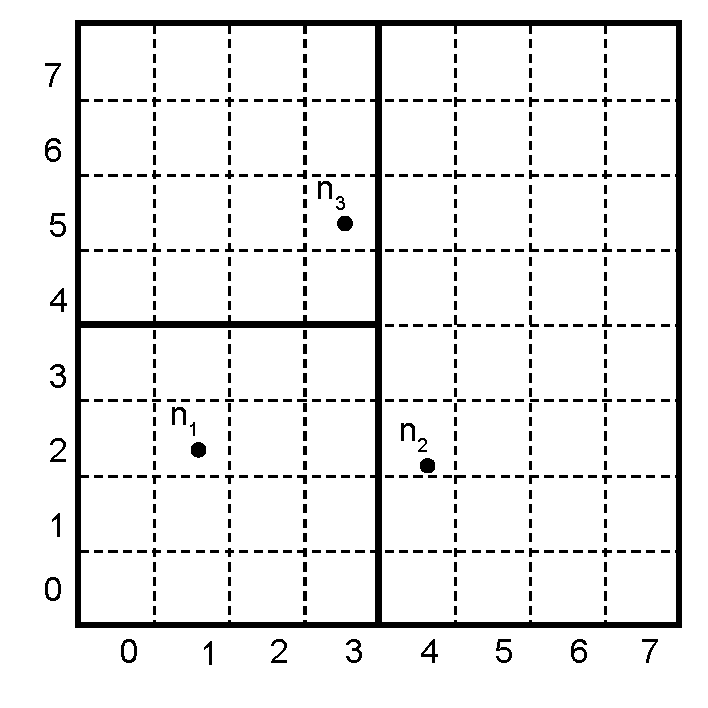
\includegraphics[width=1.0\textwidth]{can3}
\end{figure}
\end{column}
\end{columns}
		
\end{frame}	

%-------------------------------------------------------------------------
\begin{frame}{Example: 2-dimensional space}

\begin{columns}
\begin{column}{0.5\textwidth}
\structure{Example}:\\
\BI
\item Nodes $n_4:(5, 5)$ and $n_5:(6,6)$ join
\EI
\end{column}
\begin{column}{0.5\textwidth}
\begin{figure}
	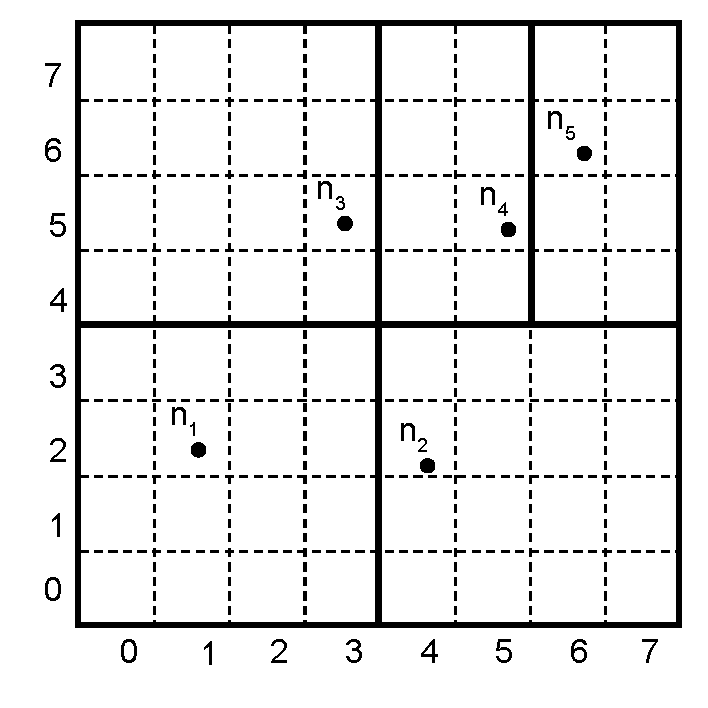
\includegraphics[width=1.0\textwidth]{can4}
\end{figure}
\end{column}
\end{columns}
		
\end{frame}	


%-------------------------------------------------------------------------
\begin{frame}{Example: 2-dimensional space}

\begin{columns}
\begin{column}{0.5\textwidth}
\structure{Example}:\\
\BI
\item Nodes: $n_1:(1, 2)$, $n_2:(4,2)$, $n_3:(3, 5)$, $n_4:(5,5)$, $n_5:(6,6)$
\item Items: $k_1:(2,3)$, $k_2:(5,1)$, $k_3:(2,1)$, $k_4:(7,5)$
\item Each item is stored by the node who owns its mapping in the space
\EI
\end{column}
\begin{column}{0.5\textwidth}
\begin{figure}
	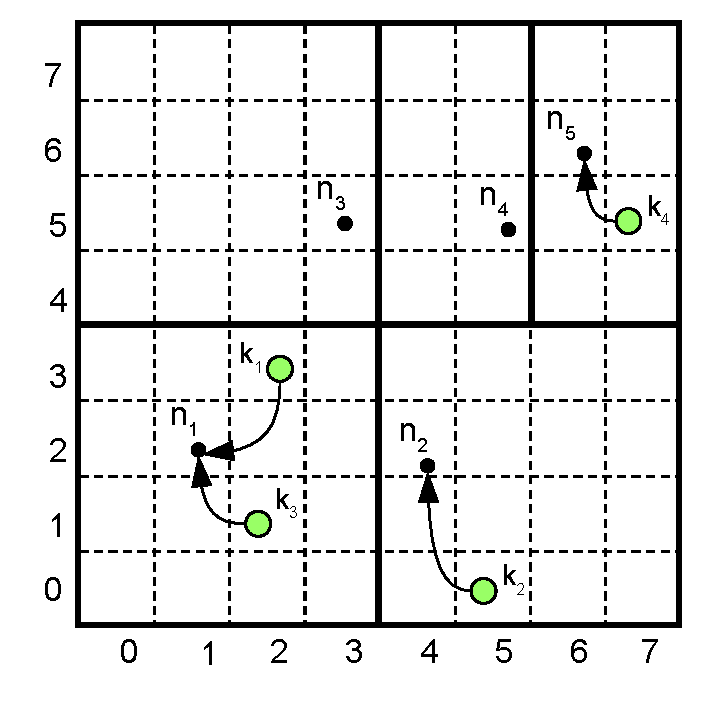
\includegraphics[width=1.0\textwidth]{can5}
\end{figure}
\end{column}
\end{columns}
		
\end{frame}	

%-------------------------------------------------------------------------
\begin{frame}{Example: 2-dimensional space}

\begin{columns}
\begin{column}{0.5\textwidth}
\structure{Example}:\\
\BI
\item Each node knows its neighbors in the $d$-space
\item Forward query to the neighbor that is closest to the query id
\item Example: assume $n_1$ queries $k_4$
\item Can route around some failures
\EI
\end{column}
\begin{column}{0.5\textwidth}
\begin{figure}
	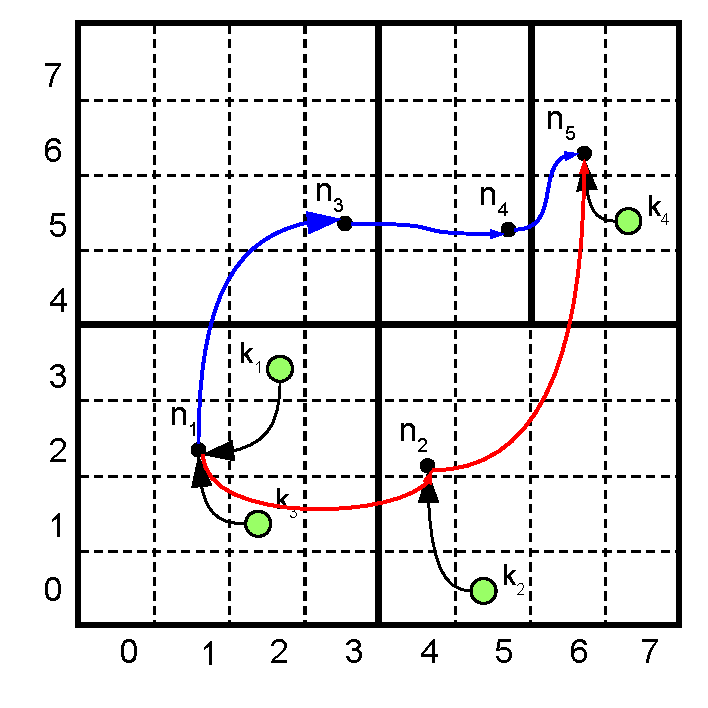
\includegraphics[width=1.0\textwidth]{can6}
\end{figure}
\end{column}
\end{columns}
		
\end{frame}	

%-------------------------------------------------------------------------
\begin{frame}{Example: 2-dimensional space}

\begin{columns}
\begin{column}{0.5\textwidth}
\structure{Node joining}:\\
\BE
\item Discover some node $I$ already in CAN
\item Pick random point $(x,y)$ in space
\item $I$ routes to $(x,y)$, discovers node $J$ 
\EE
\end{column}
\begin{column}{0.5\textwidth}
\begin{figure}
	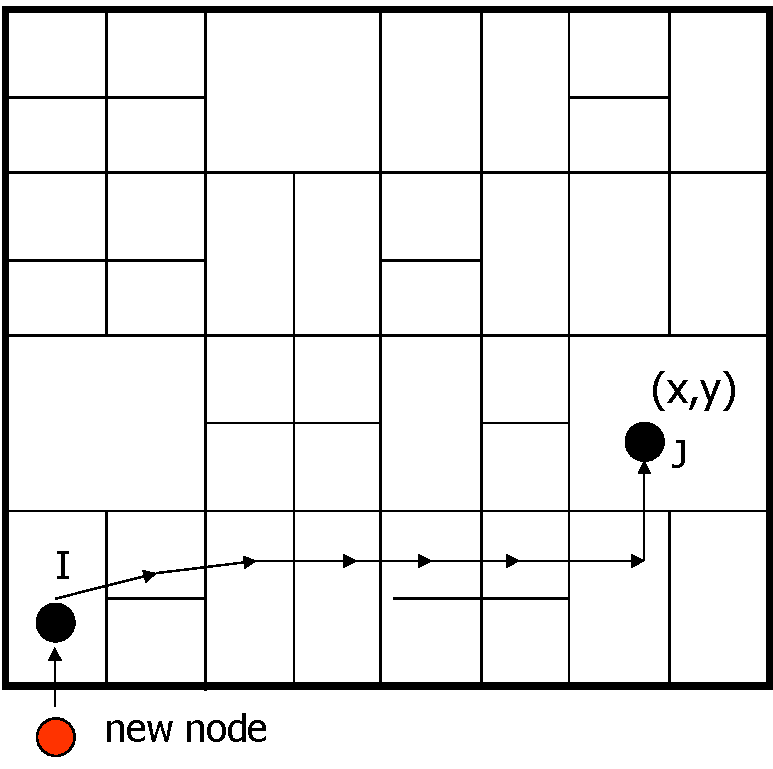
\includegraphics[width=1.0\textwidth]{can-join1}
\end{figure}
\end{column}
\end{columns}

\end{frame}

%-------------------------------------------------------------------------
\begin{frame}{Example: 2-dimensional space}

\begin{columns}
\begin{column}{0.5\textwidth}
\structure{Node joining}:\\
\BE
\item Split $J$ zone in half
\item New node owns one half
\EE
\end{column}
\begin{column}{0.5\textwidth}
\begin{figure}
	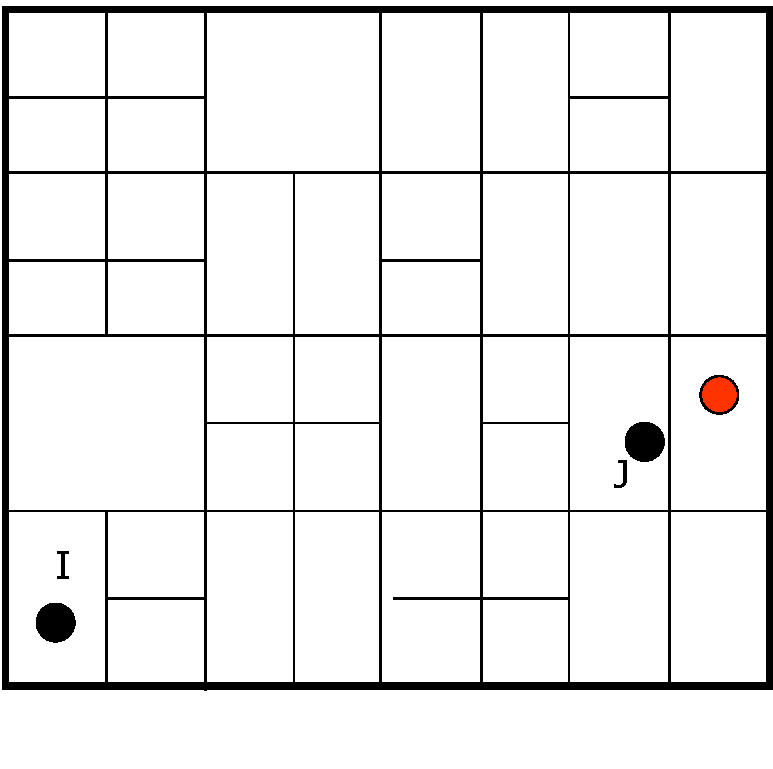
\includegraphics[width=1.0\textwidth]{can-join2}
\end{figure}
\end{column}
\end{columns}

\end{frame}

%-------------------------------------------------------------------------
\begin{frame}{Node departures}

\structure{Take-over mechanism}:
\BIL
\item Node explicitly hands over its zone and the associated (key,value) database to one of its neighbors
\item A maximum of $2d$ nodes need to be contacted
\item Problem: in case of network failure, no regeneration of data
\item Solution: every node has a backup of its neighbors 
\EIL
	
\end{frame}


%-------------------------------------------------------------------------
\begin{frame}{Multi-verse?}

\structure{Increasing availability}:
\BIL
\item Each key is mapped into $r$ different \alert{realities}
\item Each reality is associated with a different hash function
\item A key is not available only when the $r$ nodes hosting it in different
  realities are down at the same time
\EIL
	
\end{frame}


%%%%%%%%%%%%%%%%%%%%%%%%%%%%%%%%%%%%%%%%%%%%%%%%%%%%%%%%%%%%%%%%%%%%%%%%%%

\subsection{Kademlia}

%-------------------------------------------------------------------------
\begin{frame}{Kademlia}
	
\structure{Key points}\\
\BI
\item Kademlia uses tree-based routing
\item SHA-1 hash function in a $160$-bit address space
\item Every node maintains information about keys \alert{close} to itself 
	\BI
	\item Distance based on the XOR metric: $d(a,b) = a \oplus b$
	\EI
\item Uses parallel asynchronous queries to avoid timeout delays
\item Routes are selected based on latency
\EI

\begin{Bib}
{\scriptsize
	\bibentry{maymounkov2002kpp}
}
\end{Bib}
	
	
\end{frame}

%-------------------------------------------------------------------------
\begin{frame}[t]{Kademlia Tree}

\begin{figure}
	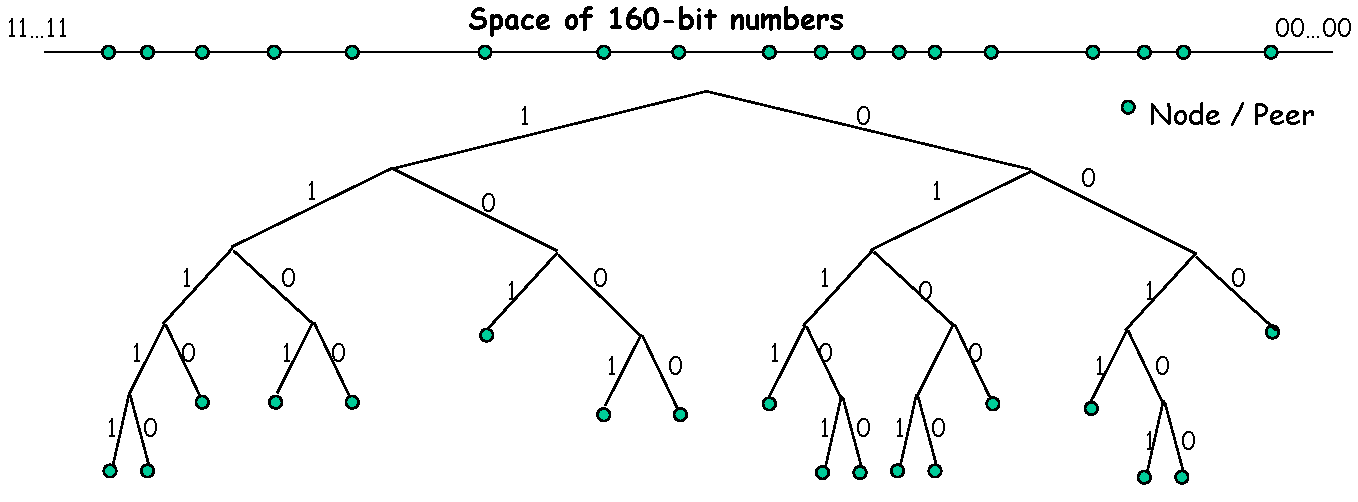
\includegraphics[width=\textwidth]{kad1}
\end{figure}

\BI
\item Nodes are treated as leafs in binary tree
\item Node's position in the tree is determined by the \alert{shortest unique} prefix of its ID
\item A node is responsible for all “closest” IDs (those having same prefix as itself)
\EI

\end{frame}

%-------------------------------------------------------------------------
\begin{frame}[t]{Kademlia Tree}

\begin{figure}
	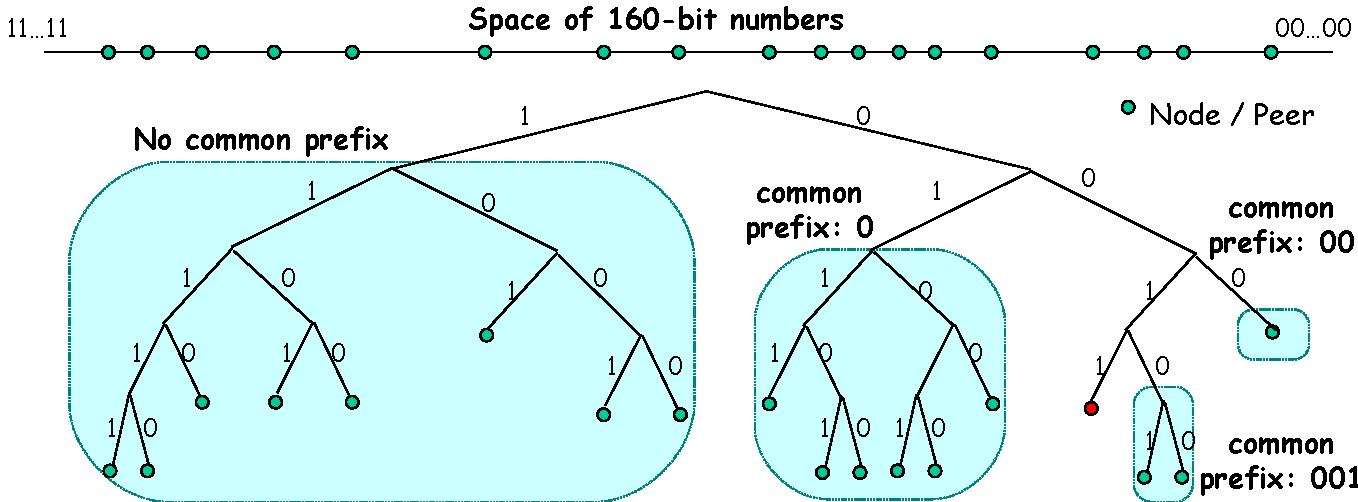
\includegraphics[width=\textwidth]{kad2}
\end{figure}

\BI
\item From the point of view of each node, the tree is divided into a series of maximal subtrees that do not contain the node
\item Example: the red node with prefix \texttt{0011}
\item A node must know at least one node in each of these subtrees
\EI

\end{frame}

%-------------------------------------------------------------------------
\begin{frame}[t]{Routing table}

\begin{figure}
	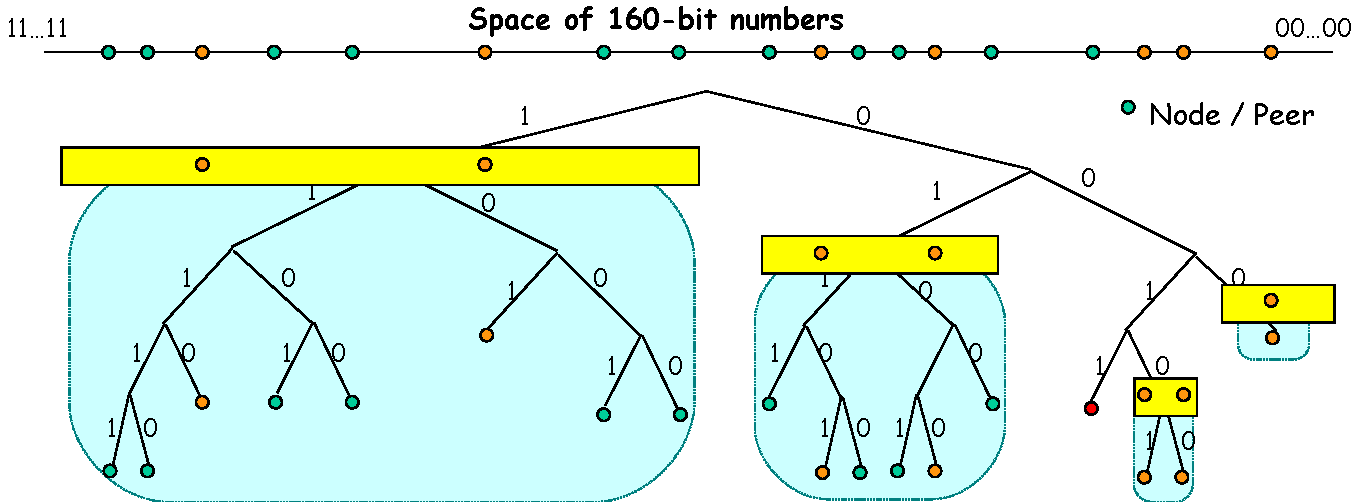
\includegraphics[width=\textwidth]{kad4}
\end{figure}

\BI
\item Consider routing table for a node with prefix \texttt{0011}
\item The routing table is composed of a series of \alert{$k$-buckets} corresponding to each of the subtrees
\item Consider a $2$-bucket example, each bucket will have at least $2$ contacts for each subtree
\EI

\end{frame}

%-------------------------------------------------------------------------
\begin{frame}[t]{Kademlia Tree}

\begin{figure}
	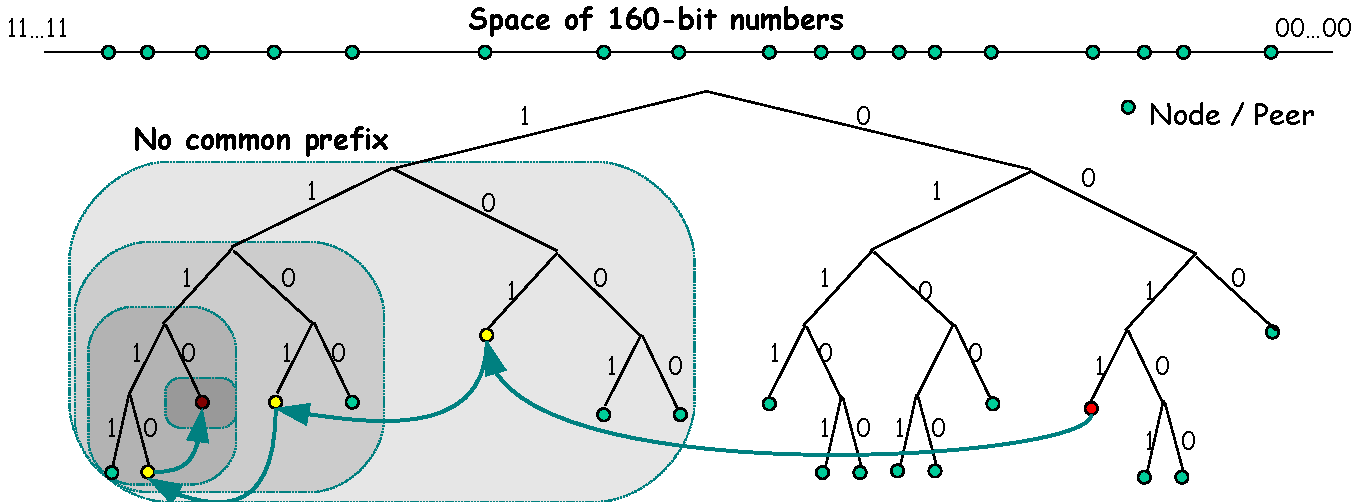
\includegraphics[width=\textwidth]{kad3}
\end{figure}

\BI
\item Consider a query for ID \texttt{\alert{1110}10}\ldots initiated by node \texttt{\alert{0011}100}\ldots
\EI

\end{frame}

%-------------------------------------------------------------------------
\begin{frame}{Messages}
	
Kademlia protocol consists of 4 RPCs:
\BIL
\item \alert{$\mathit{ping}_{n \rightarrow m}()$}
	\BI
	\item Probe node $m$ to see if it is online
	\EI
\item \alert{$\mathit{store}_{n \rightarrow m}(k, v)$}
	\BI
	\item Instruct node $m$ to store a $\langle k, m \rangle$ pair
	\EI
\item \alert{$\mathit{findNode}_{n \rightarrow m}(t)$}
	\BI
	\item Returns the $k$ contacts “closest” to $t$
	\EI
\item \alert{$\mathit{findValue}_{n \rightarrow m}(k)$}
	\BI
	\item Returns the value associated to $k$, if present, or 
	\item Returns $k$ contacts closest to $k$
	\EI
\EIL
	
\end{frame}

\begin{frame}{Routing}

\structure{Goal: find $k$ nodes closest to ID $t$ -- Protocol executed by $n_0$}
\begin{columns}
\begin{column}{0.65\textwidth}
\BI
\item \alert{Initial phase} :
	\BI
	\item insert in a set $S$ all the nodes in the routing table
	\EI
\item \alert{Iteration}
	\BI
	\item select a subset $T \subseteq S$ of the $\alpha$ nodes closest to $t$
	\item invoke $\mathit{findNode}(t)$ on nodes in $T$, \alert{in parallel}
	\item collect the replies in a new set $S$
	\item repeat until no new node is discovered 
	\EI
\item \alert{Final phase}
	\BI
	\item invoke $\mathit{findNode}(t)$ to all of $k$ closest nodes not already queried
	\item return when have results from all the $k$-closest nodes
	\EI
\EI
\end{column}
\begin{column}{0.35\textwidth}
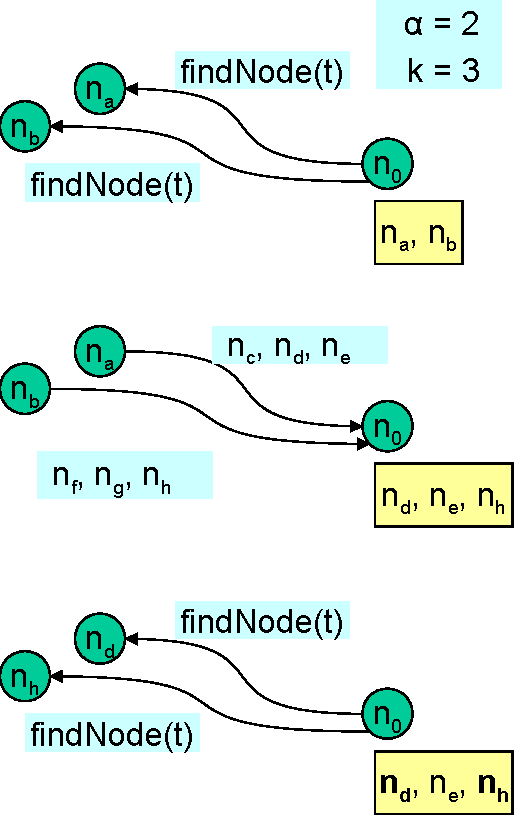
\includegraphics[width=\textwidth]{kad-routing}
\end{column}
\end{columns}

\end{frame}


%-------------------------------------------------------------------------
\begin{frame}{Kademlia summary}
	
\structure{Strengths}:\\
\BI
\item Low control message overhead
\item Tolerance to node failure and leave
\item Capable of selecting low-latency path for query routing
\item Unlike Chord, Kademlia is symmetric: $a \oplus b = b \oplus a$
\BI
\item Peers receive lookup queries from precisely the same set of neighbors contained in their routing tables
\EI
\EI

\smallskip
\structure{Weaknesses}:
\BI
\item Balancing of storage load is not truly solved
\item No experimental results provided
\EI


\end{frame}

%%%%%%%%%%%%%%%%%%%%%%%%%%%%%%%%%%%%%%%%%%%%%%%%%%%%%%%%%%%%%%%%%%%%%%%%%%
\subsection{Cassandra}

%-------------------------------------------------------------------------
\begin{frame}{Cassandra}
Few information available:\\
\BIL
\item $O(1)$ routing hops
\item $O(N)$ routing state
\BI
\item Thanks to a routing protocol that guarantees that eventually
every node knows every other node
\EI
\EIL

\begin{Bib}
{\scriptsize
	\bibentry{cassandra}
}
\end{Bib}
\end{frame}

%%%%%%%%%%%%%%%%%%%%%%%%%%%%%%%%%%%%%%%%%%%%%%%%%%%%%%%%%%%%%%%%%%%%%%%%%%
\subsection{DHT Security}

%-------------------------------------------------------------------------
\begin{frame}{Security aspects of DHTs}

\begin{block}{Security weaknesses specific to DHTs}
\BI
\item \alert{Sybil} attacks
	\BI
	\item an attacker introduces a large number of bogus nodes that can subvert protocols based on redundancy
	\EI
\item \alert{Eclipse} attacks
	\BI 
	\item an attacker tries to corrupt the routing tables of honest nodes by filling them with references to malicious nodes
	\EI
\item \alert{Routing} and \alert{storage} attacks 
	\BI
	\item various attacks where malicious nodes do not follow the routing and storage protocols correctly
	\EI
\EI
\end{block}

\smallskip
\begin{Bib}
{\scriptsize
	\bibentry{dht-security}
}
\end{Bib}

\end{frame}

%-------------------------------------------------------------------------
\begin{frame}{Example of attacks}
	
\begin{figure}
	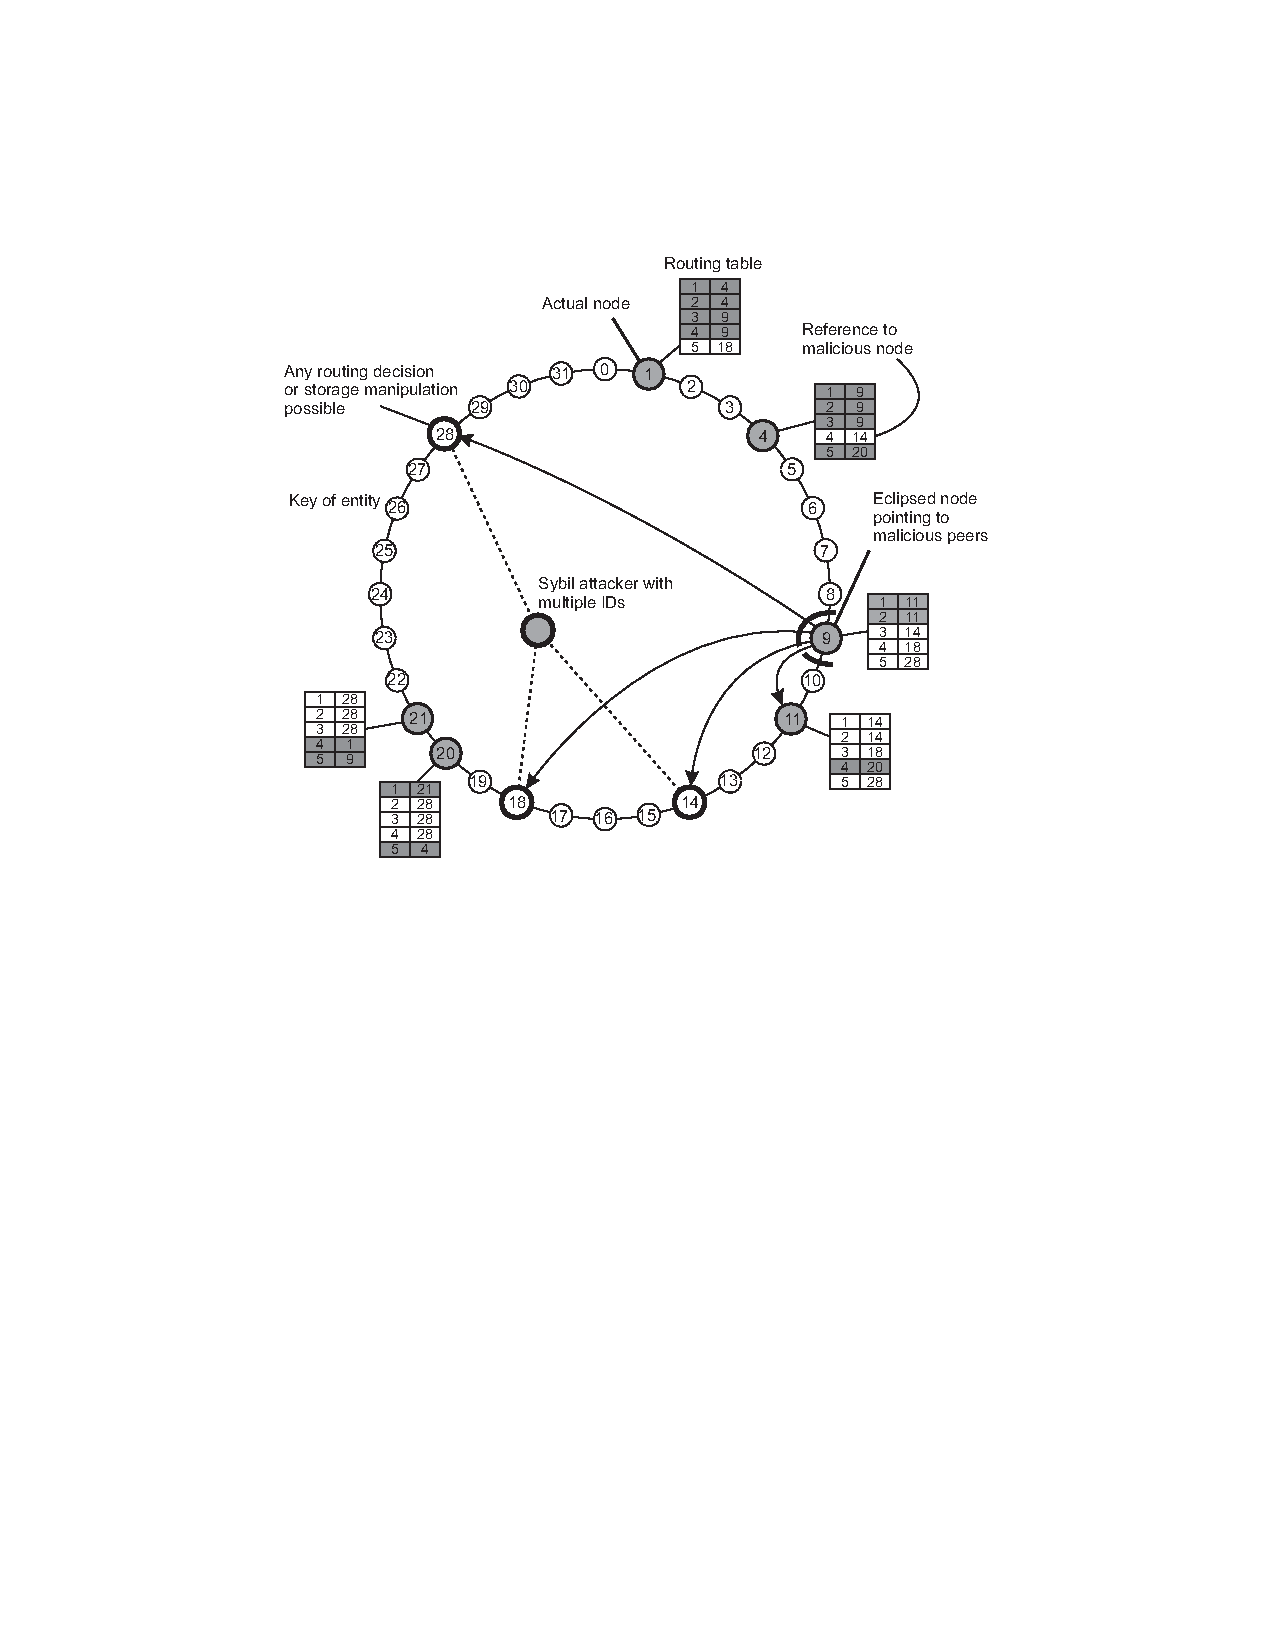
\includegraphics[width=0.7\textwidth]{dht-security}
\end{figure}

\end{frame}


%-------------------------------------------------------------------------
\begin{frame}{Defenses against Sybil attacks}

\BIL
\item Collusion is easier 
\item Possible defenses:
	\BI
	\item Centralized certification
	\item Distributed registration
	\item Physical network characteristics
	\item Social networks
	\item Computational puzzles
	\EI
\item You can only reduce the impact of Sybil attacks, not eliminate them
completely
\EIL

\end{frame}

%-------------------------------------------------------------------------
\begin{frame}{Defenses against eclipse attacks}

\BIL
\item Effect of eclipse attack (“\alert{table poisoning}”) is measured by:
\[
  \frac{
    \textrm{percentage of malicious entries in routing tables}}{
	\textrm{percentage of malicious users in the network}
   }
\]
\item Possible defenses:
\BI
\item Constrained neighbor selection
  \BI
  \item Original Chord: only one node may fit in a finger table entry -- good
  \item Random Chord: several nodes may fit in finger table entry -- bad
  \item Pastry: some table entries may be filled by any node sharing a short prefix -- bad
  \item Kademlia: table entries are filled by fast-responding peers -- good
  \EI
\item In-degree anonymous auditing
  \BI
  \item Malicious nodes have larger in-degree
  \EI
\EI

\EIL

\end{frame}

%-------------------------------------------------------------------------
\begin{frame}{Defenses against routing and storage attacks}

\BIL
\item \alert{Redundant routing}
  \BI
  \item Possible approaches:
	  \BI
	  \item Multiple paths
	  \item Wide paths
	  \item Multiple wide paths
	  \EI
  \item Wide paths require one good node per hop, multiple paths require
    a path with only good nodes
  \EI
\item \alert{Redundant storage} 
  \BI
  \item Storing replicas “numerically close” to each other
    \BI
       \item Chord, Pastry, Kademlia
	   \item Pros: easier to maintain consistency
	   \item Cons: malicious node may control a region of space
    \EI
  \item Storing replicas spread over the identifier space
    \BI
       \item Tapestry, several other proposals
       \item Pros: most difficult to subvert an area
       \item Cons: requires additional tables
    \EI
  \EI
\EIL

\end{frame}

%-------------------------------------------------------------------------
\begin{frame}{Why Kademlia?}

\structure{Generic reasons}
\BI
\item Relative security: wide searches
\item Replicated storage
\EI

\smallskip
\structure{The reality is that Kademlia is insecure}
\BI
\item Successful (academic) attacks on Kad/BitTorrent
\item Successful infiltrations on the Storm BotNet
\EI

\smallskip
\structure{The real reasons}
\BI
\item For BitTorrent, damage is limited anyway (decentralized tracking)
\item Many alternative ways to obtain peers (PEX, multiple trackers)
\EI


\end{frame}


%%%%%%%%%%%%%%%%%%%%%%%%%%%%%%%%%%%%%%%%%%%%%%%%%%%%%%%%%%%%%%%%%%%%%%%%%%
\subsection{DHT Summary}

%-------------------------------------------------------------------------
\begin{frame}{Comparison}

\begin{table}
\begin{tabular}{|l||c|c|c|c|c|c|c|c|}
\hline
   & \textbf{CAN} & \textbf{Chord} & \textbf{Tapestry} & \textbf{Pastry}  \\
\hline\hline
Architecture & $d$-dimens. & ring & Plaxton & Plaxton \\
             & space           &      & tree    & tree  \\
\hline
Routing hops & $O(dN^{1/d})$ & $O(\log N)$ & $O(\log_b N)$ & $O(\log_b N)$ \\
\hline
Routing state & $2d$ & $\log N$ & $\log_b N$ & $B\log_b N$\\
\hline
Join cost & $2d$ & $(\log N)^2$ & $\log_b N$ & $\log_b N$ \\
\hline
\end{tabular}
\end{table}

\begin{table}
\begin{tabular}{|l||c|c|c|c|c|c|c|c|}
\hline
   & \textbf{Kademlia} & \textbf{Viceroy} & \textbf{Koorde} & \textbf{Kelips} \\
\hline\hline
Architecture & Tree & Butterfly & de Brujin & $n$-dimens. \\
             &      & network   & graph     & space \\
\hline
Routing hops & $O(\log N)$ & $O(\log n)$ & $O\left(\frac{\log n}{\log \log n}\right)$ & $O(1)$ \\
\hline
Routing state & $k\log N$ & $\log N$ & $\log N$ & $\sqrt{n}$ \\
\hline
Join cost & $k \log N$ & $\log N$ & $\log N$ & $\sqrt{n}$ \\
\hline
\end{tabular}
\end{table}

\end{frame}

%-------------------------------------------------------------------------
\begin{frame}{Conclusions}

\BIL
\item The DHT abstraction is doing well, both inside clouds and in 
P2P networks
\item Kademlia seems to be the winner. Main reasons:
\BI
\item Performance
\item Relative security
\EI
\EIL

\end{frame}



%%%%%%%%%%%%%%%%%%%%%%%%%%%%%%%%%%%%%%%%%%%%%%%%%%%%%%%%%%%%%%%%%%%%%%%%%%
\section{Unstructured systems}

\subsection{Gnutella}

%-------------------------------------------------------------------------
\begin{frame}{Gnutella: brief history}
	
\BIL
\item Nullsoft (a subsidiary of AOL) released Gnutella on March 14th, 2000,
  announcing it on Slashdot
\item AOL removed Gnutella from Nullsoft servers on March 15th, 2000
\item After a few days, the Gnutella protocol was reverse-engineered
\item Napster was shutdown in early 2001, spurring the popularity of Gnutella
\item On October 2010, LimeWire (a popular client) was shutdown by court's order
\EIL

\end{frame}


%-------------------------------------------------------------------------
\begin{frame}{Gnutella}
	
Gnutella is a protocol for peer-to-peer \alert{search}, consisting of:\\
\BIL
\item A set of message formats 
	\BI
	\item 5 basic message types
	\EI
\item A set of rules governing the exchange of messages
	\BI
	\item Broadcast
	\item Back-propagate
	\item Handshaking
	\EI
\item An \alert{hostcache} for node bootstrap
\EIL

\end{frame}


%-------------------------------------------------------------------------
\begin{frame}{Gnutella topology: unstructured}
	
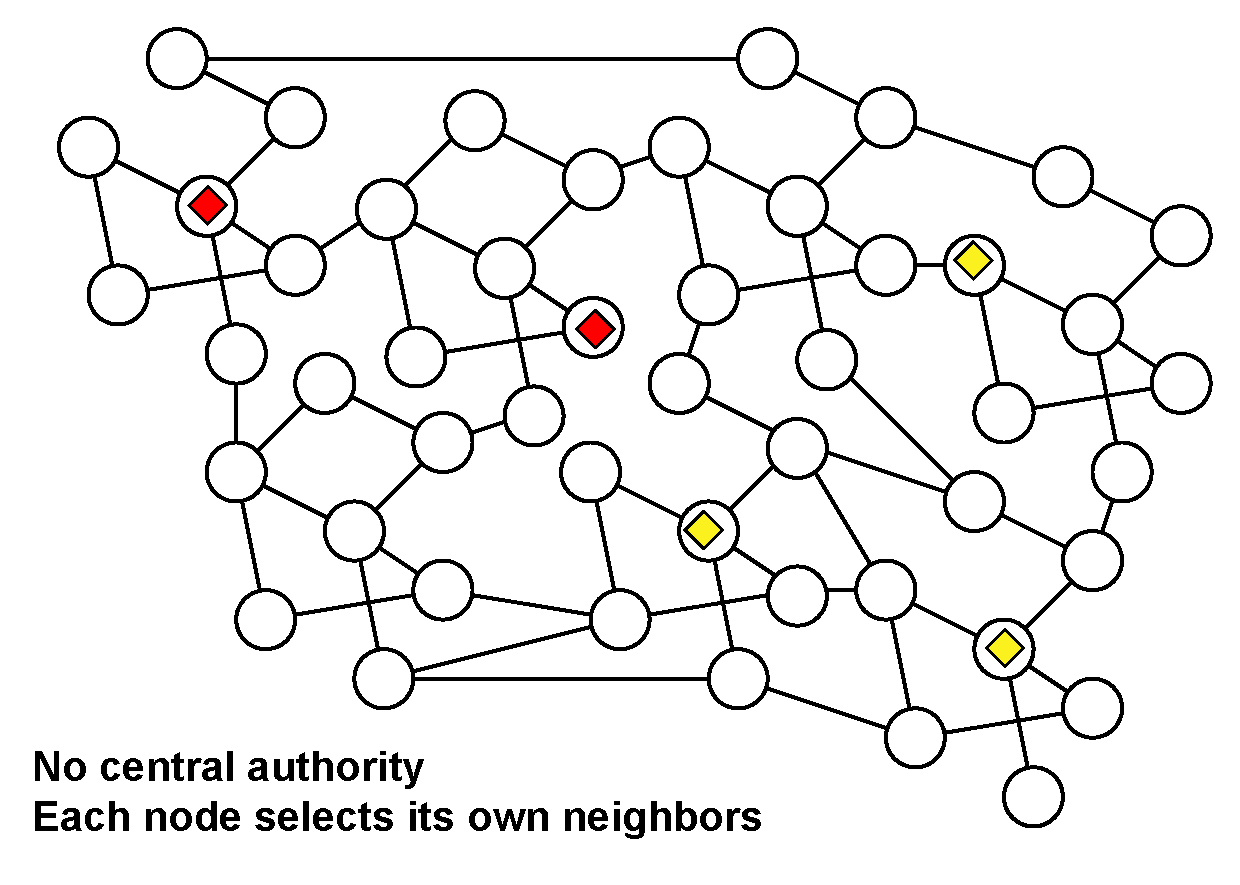
\includegraphics[width=0.9\textwidth]{gnutella1}

\end{frame}


\begin{frame}{Gnutella routing}
	
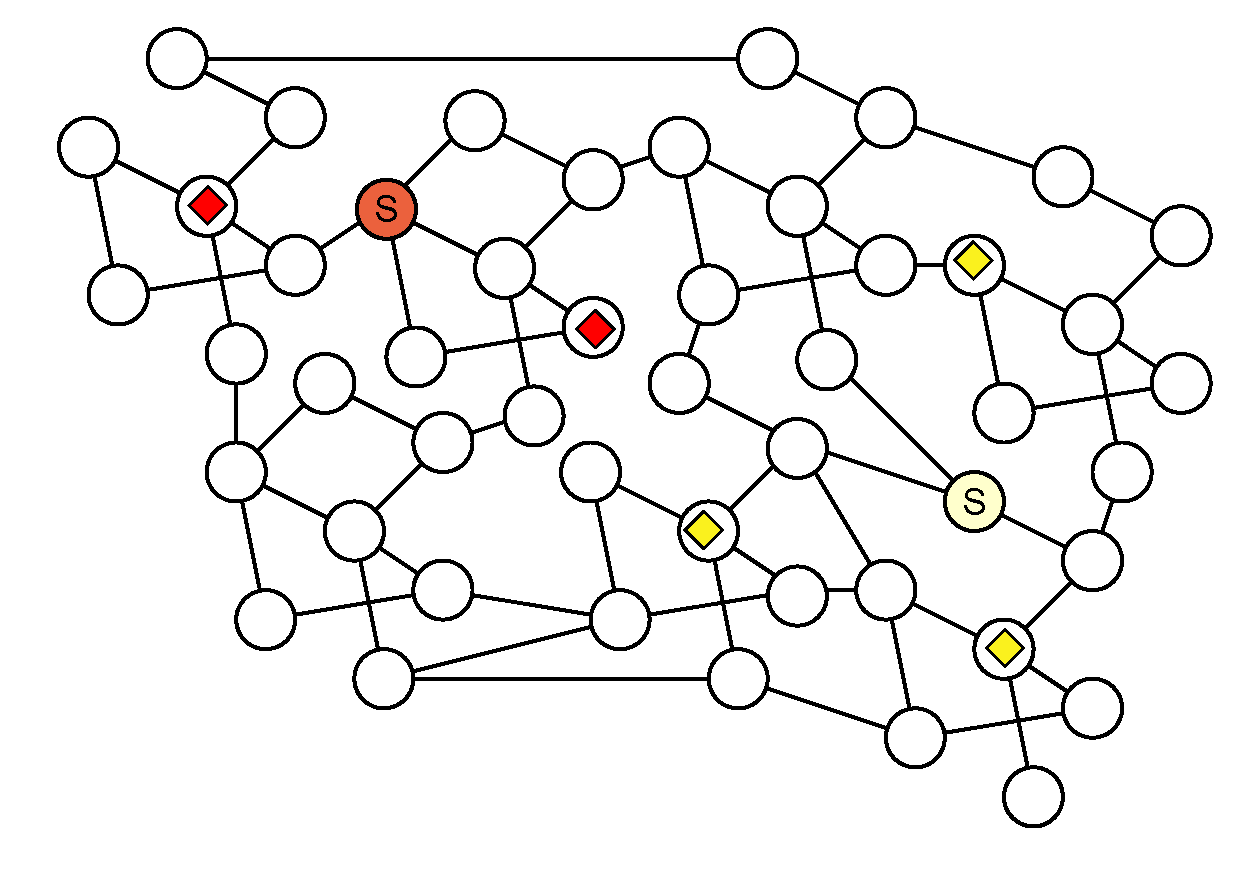
\includegraphics[width=0.9\textwidth]{gnutella2}

\end{frame}

\begin{frame}{Gnutella routing}
	
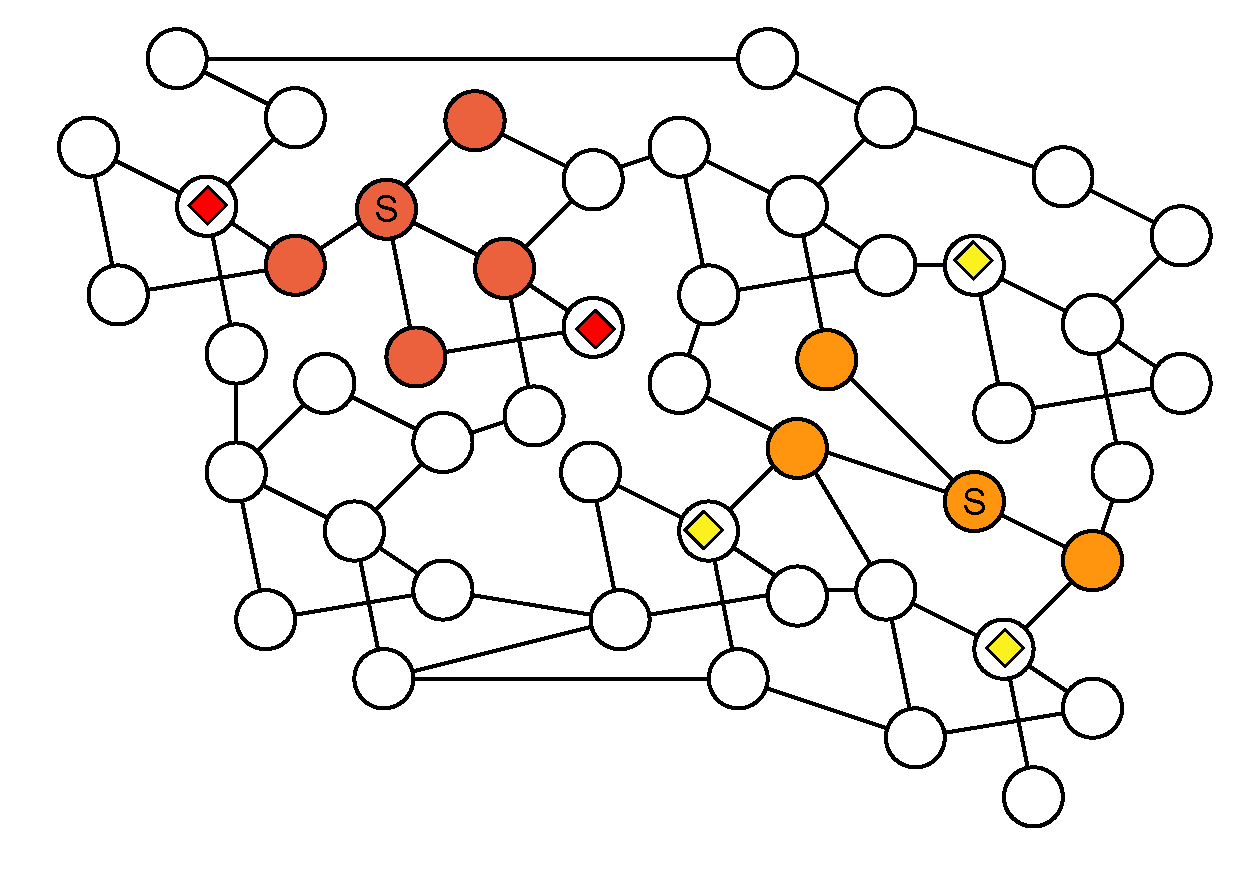
\includegraphics[width=0.9\textwidth]{gnutella3}

\end{frame}

\begin{frame}{Gnutella routing}
	
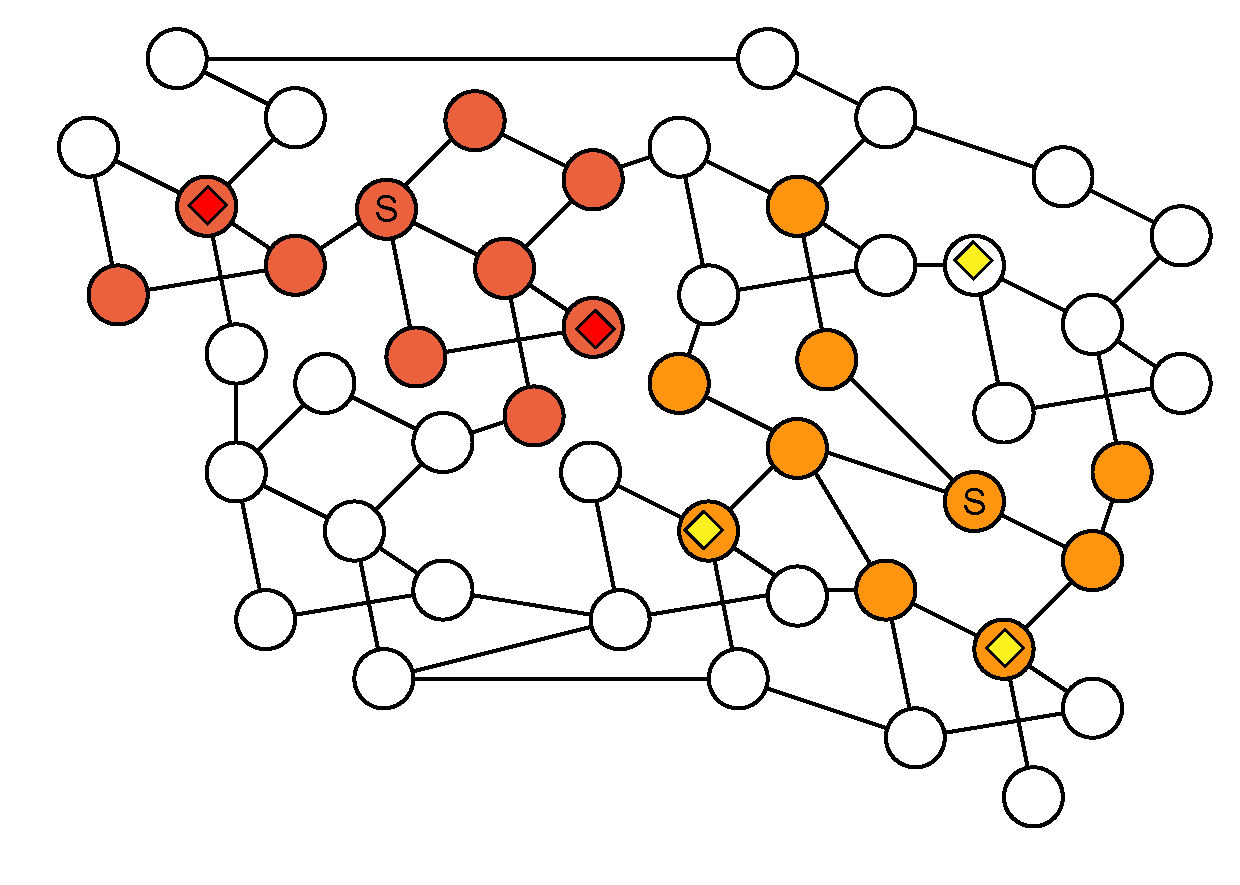
\includegraphics[width=0.9\textwidth]{gnutella4}

\end{frame}

\begin{frame}{Gnutella routing}
	
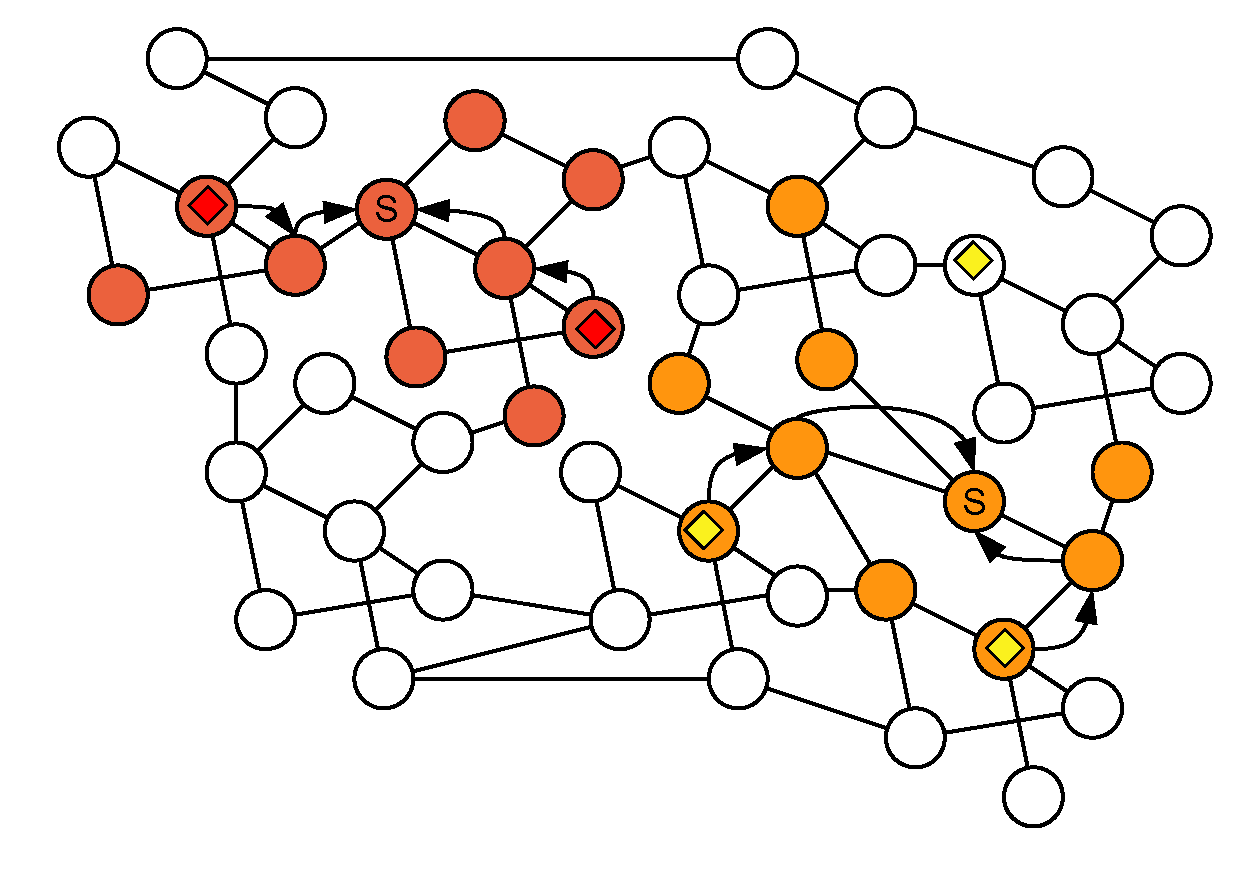
\includegraphics[width=0.9\textwidth]{gnutella5}

\end{frame}

\begin{frame}{Gnutella messages}
Each message is composed of:
\BIL
\item A 16-byte ID field uniquely identifying the message
	\BI
	\item randomly generated
	\item not related to the address of the requester (anonymity)
	\item used to detect duplicates and route back-propagate messages
	\EI
\item A message type field
	\BI
	\item \textsc{ping}, \textsc{pong}
	\item \textsc{query}, \textsc{queryhit}
	\item \textsc{push} (for firewalls)
	\EI
\item A Time-To-Live (TTL) Field
\item Payload length
\EIL

\end{frame}

\begin{frame}{Gnutella messages}

\BIL
\item \alert{\textsc{ping}} (broadcast)
	\BI
	\item Used to maintain information about the nodes currently in the network
	\item Originally, a “who's there” flooding message
	\item A peer receiving a \textsc{ping} is expected to respond with a \textsc{pong} message
	\EI
\item \alert{\textsc{pong}} (back-propagate)
	\BI
	\item A \textsc{ping} message has the same ID of the corresponding \textsc{ping} message
	\item Contains:
		\BI
		\item address of connected Gnutella peer
		\item total size and total number of files shared by this peer
		\EI
	\EI
\EIL
\end{frame}


\begin{frame}{Gnutella messages}

\BIL
\item \alert{\textsc{query}} (broadcast)
	\BI
	\item The primary mechanism for searching the distributed network
	\item Contains the query string
	\item A servent is expected to respond with a \textsc{queryhit} message if a match is found against its local data set
	\EI
\item \alert{\textsc{queryhit}} (back-propagate)
	\BI
	\item The response to a query
	\item Has the same ID of the corresponding \textsc{query} message
	\item Contains enough information to acquire the data matching the corresponding query
		\BI 
		\item IP Address + port number
		\item List of file names
		\EI
	\EI
\EIL

\end{frame}

\begin{frame}{Beyond the original Gnutella}

\structure{Several problems in Gnutella 0.4  (the original one)}:\\
\BIL
\item What kind of topology is generated?
	\BI
	\item Is it planned (“engineered”)?
	\item Is it good?
	\EI
\item \textsc{ping}-\textsc{pong} traffic
	\BI
	\item More than 50\% of the traffic generated by Gnutella 0.4 is \textsc{ping}-\textsc{pong} related
	\EI
\item Scalability
	\BI
	\item Each query generates a huge amount of traffic
	\BI
	\item e.g. $\mathit{TTL}=6, d=10 \Rightarrow 10^6$ messages 
	\EI
	\item Potentially, each query is received multiple times from all neighbors
	\EI
\EIL

\end{frame}

\begin{frame}{Gnutella overlay vs underlying topology}
	
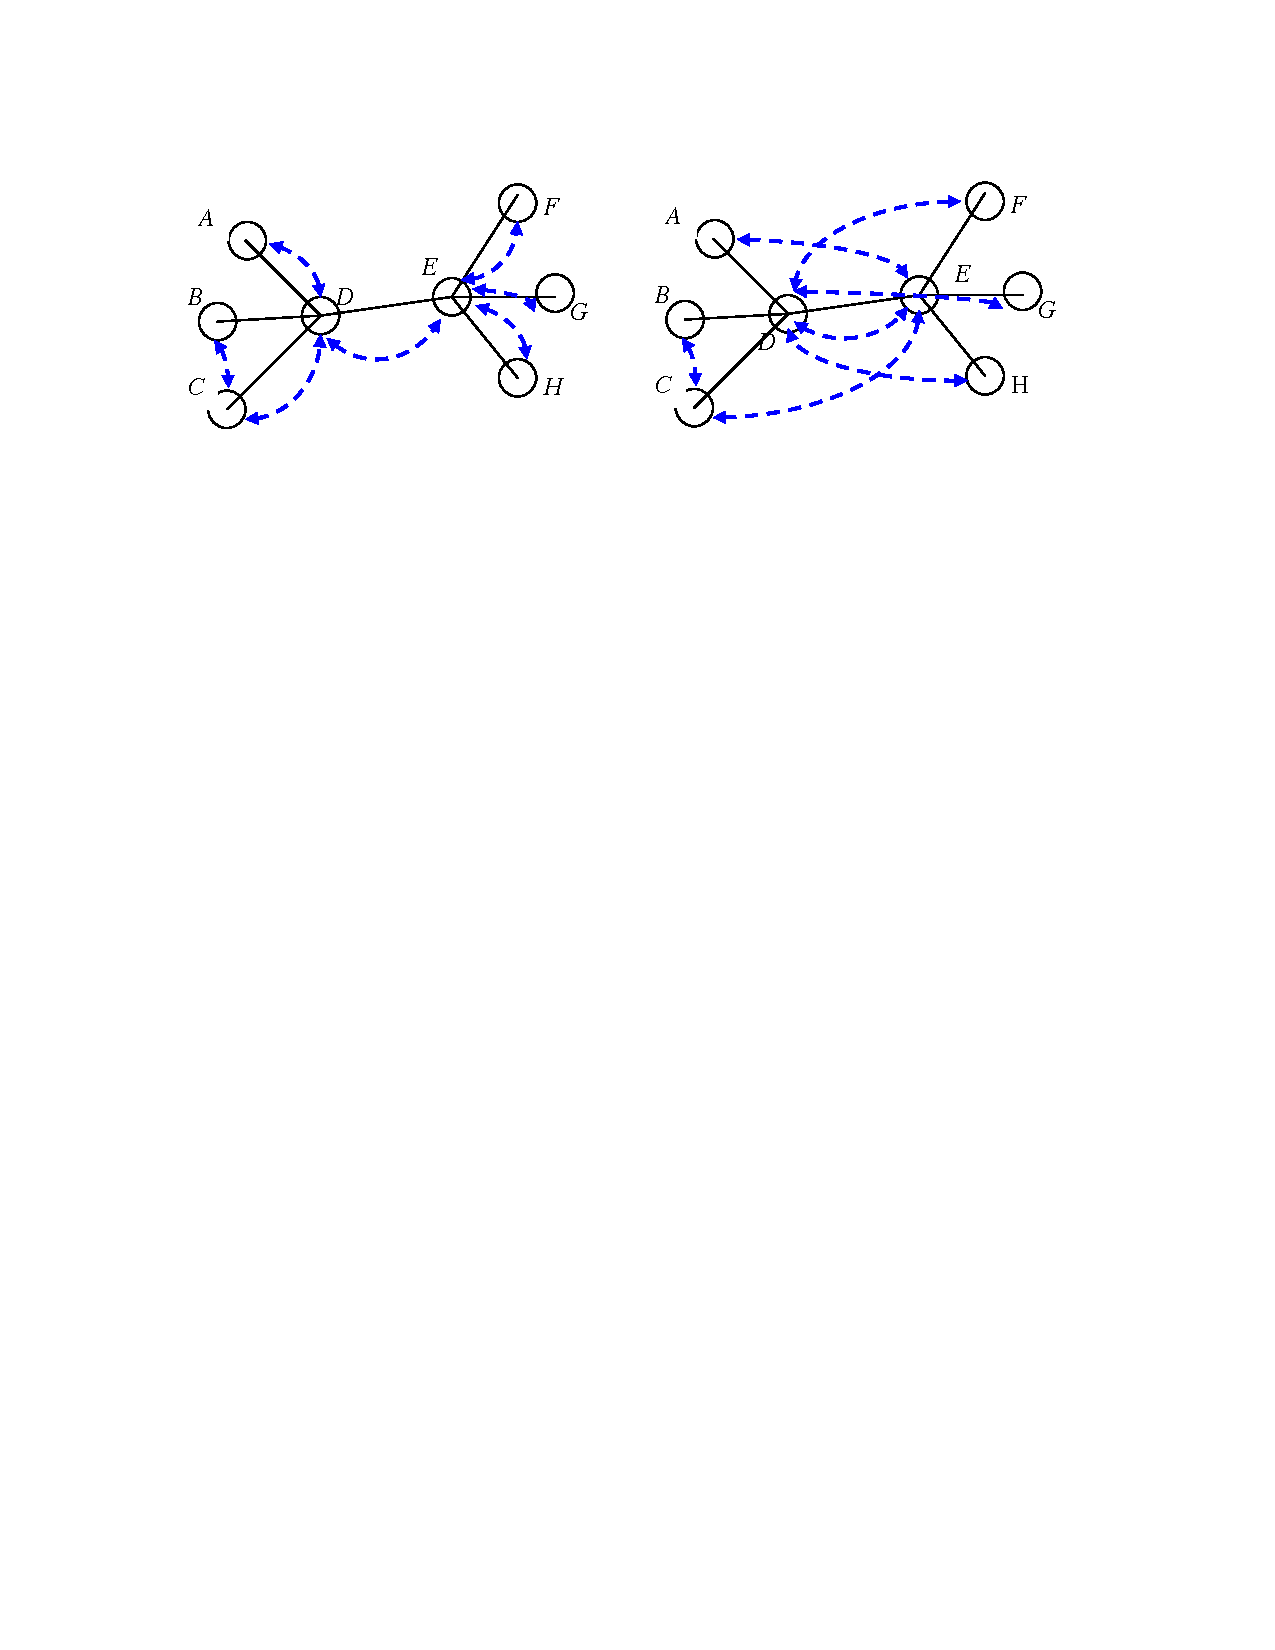
\includegraphics[width=\textwidth]{mapping3}	

\end{frame}

\begin{frame}{Traffic}
	
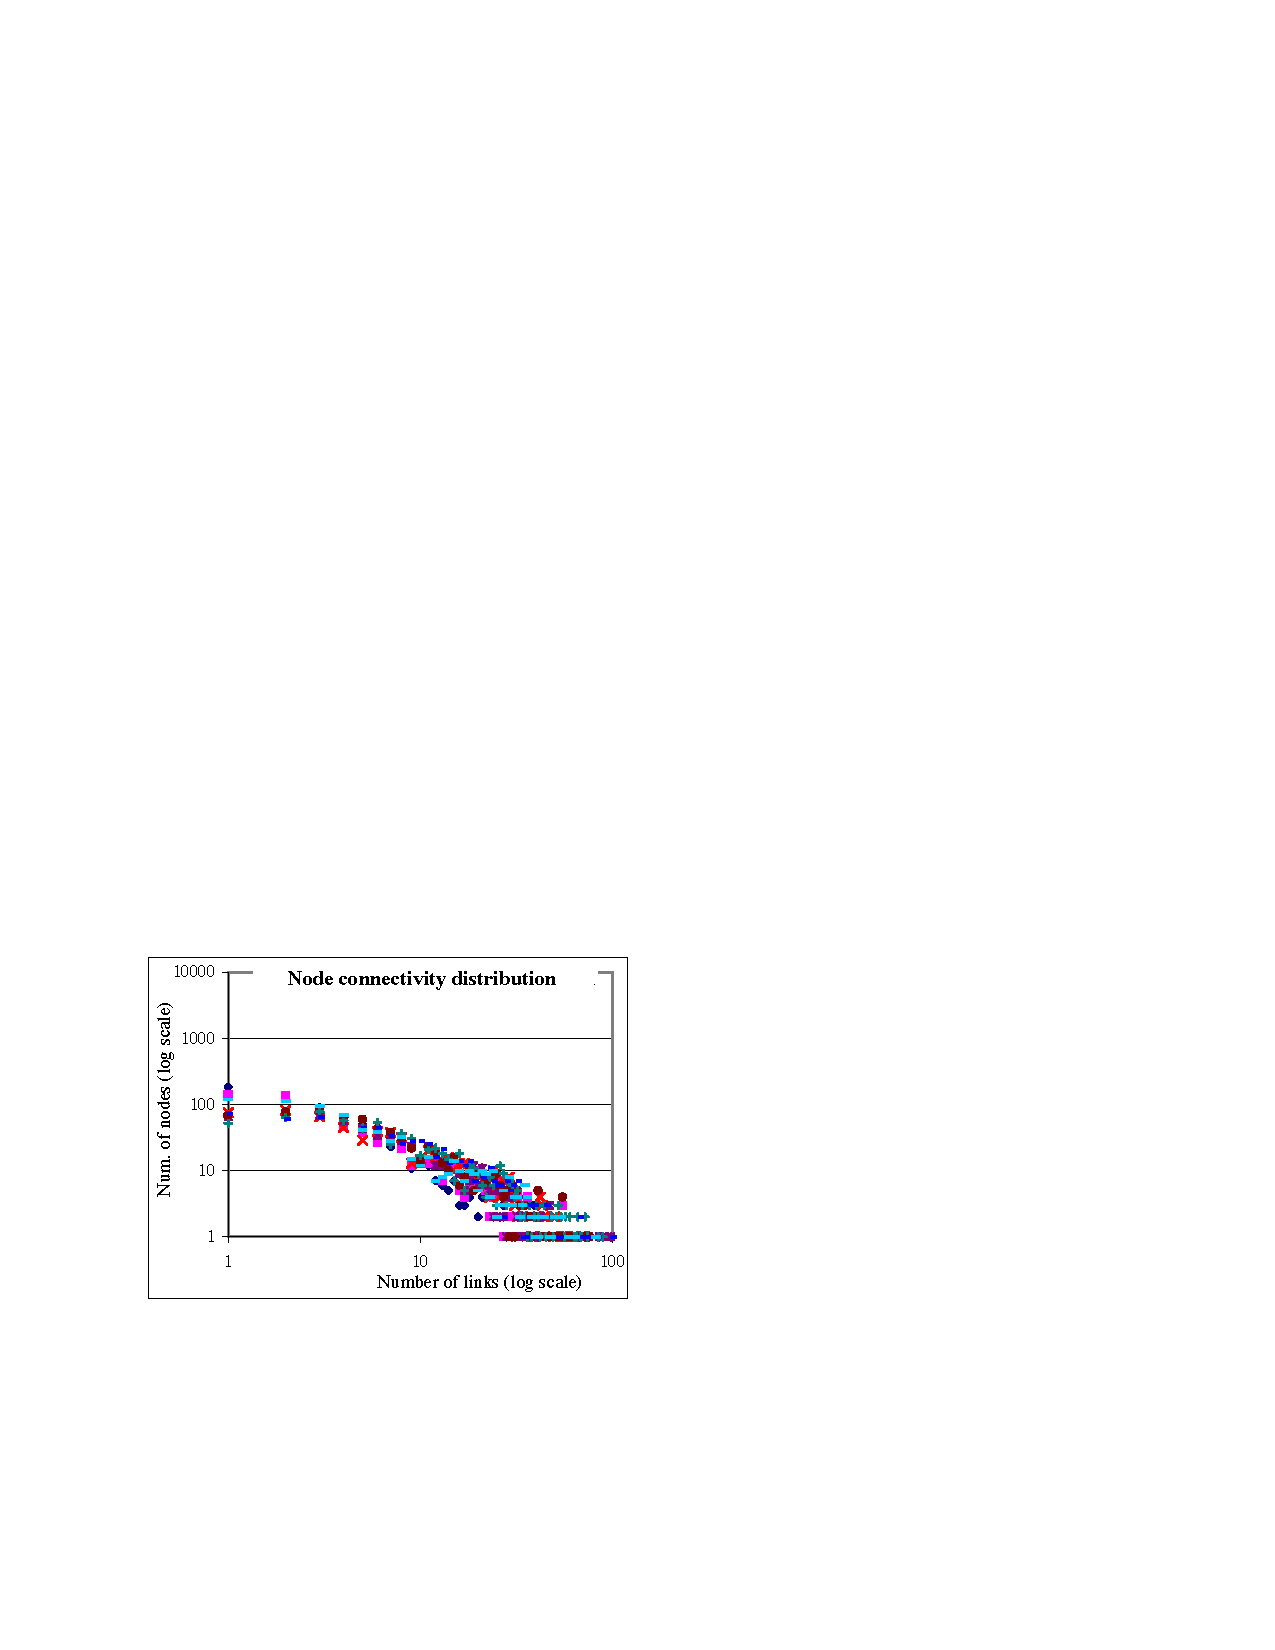
\includegraphics[width=0.8\textwidth]{mapping2}	

\end{frame}

\begin{frame}{Connectivity (and robustness)}
	
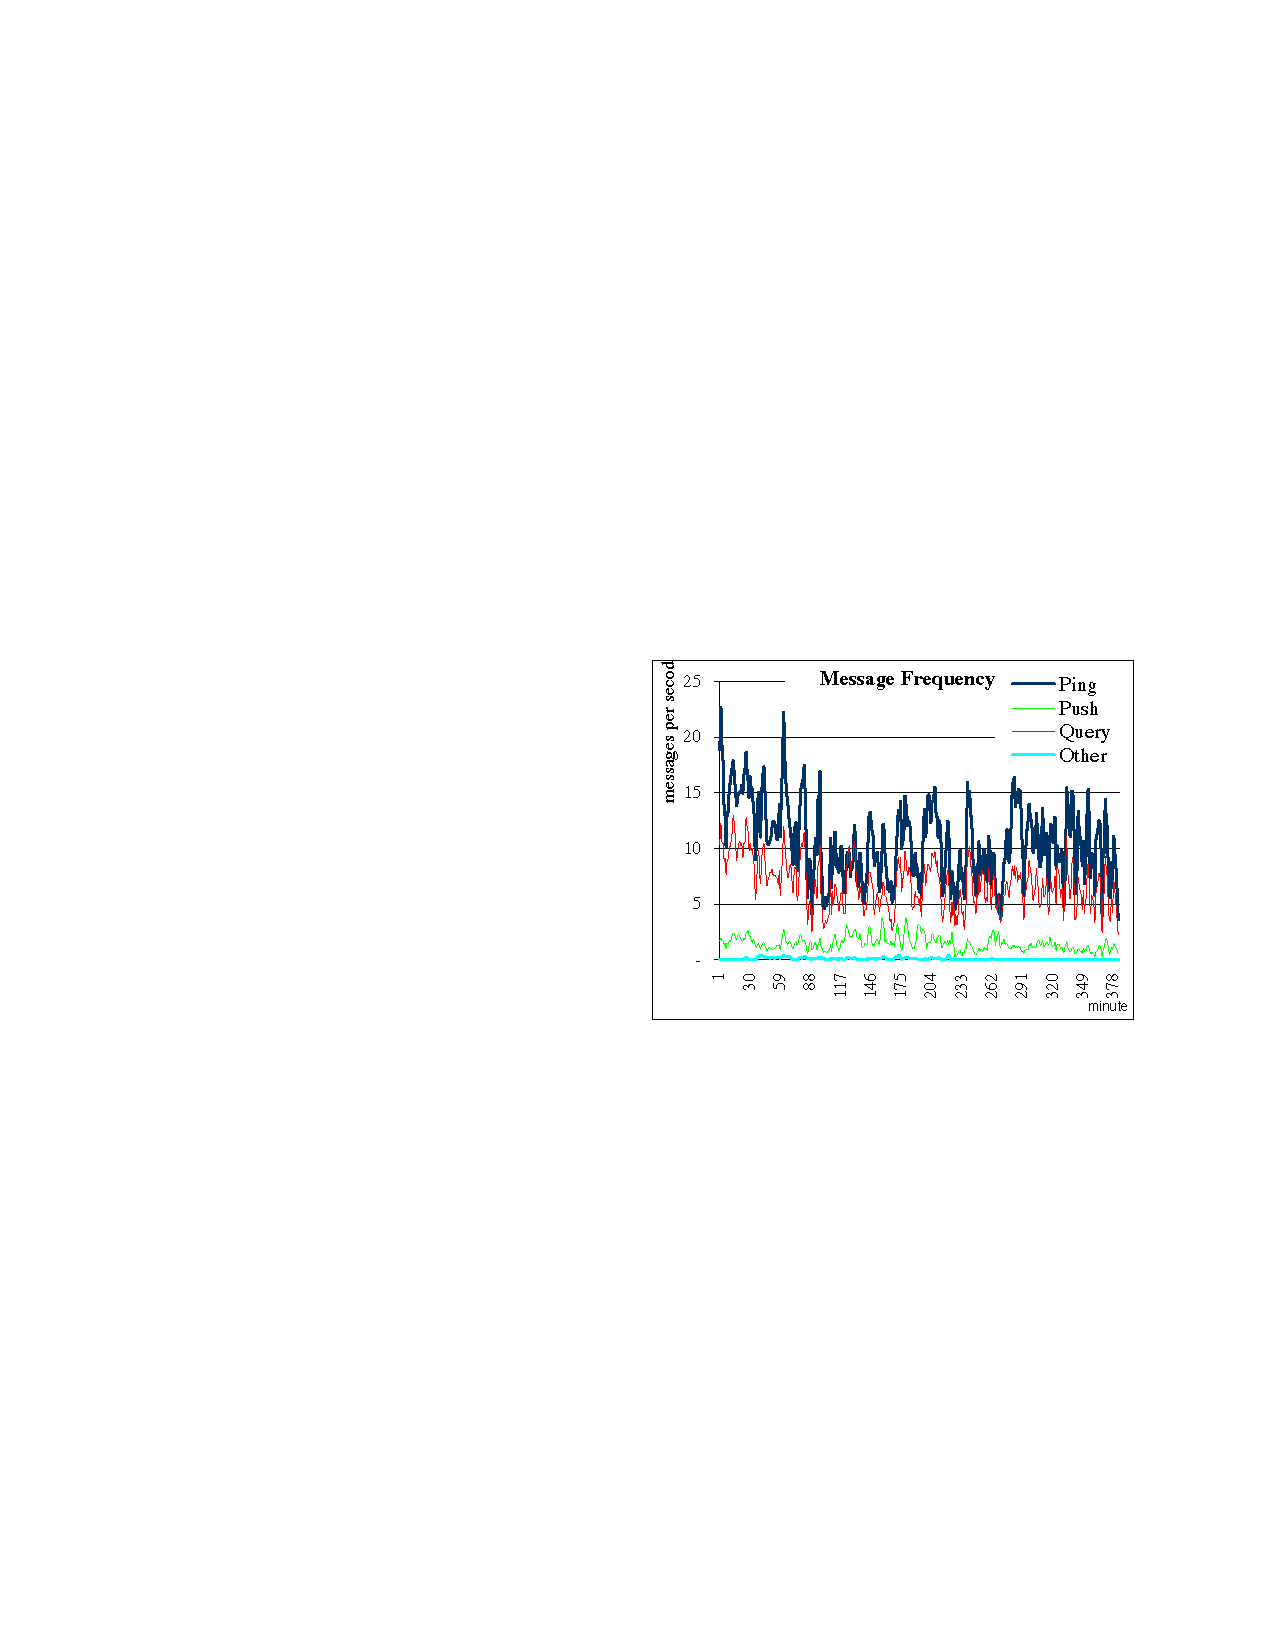
\includegraphics[width=0.8\textwidth]{mapping1}

\end{frame}

\begin{frame}{Gnutella conclusions}
	
\structure{Gnutella 0.6}:
\BI
\item Superpeer-based organization
\item Ping/pong caching
\item Query routing
\EI

\bigskip
\structure{Summary}:
\BIL
\item A milestone in P2P computing
	\BI
	\item Gnutella proved that full decentralization is possible
	\EI
\item But:
	\BI
	\item Gnutella is a patchwork of hacks
	\item The ping-pong mechanism, even with caching, is just plain inefficient
	\EI	
\EIL
\end{frame}



%%%%%%%%%%%%%%%%%%%%%%%%%%%%%%%%%%%%%%%%%%%%%%%%%%%%%%%%%%%%%%%%%%%%%%%%%%
\subsection{BitTorrent}

\begin{frame}{BitTorrent}

\BIL
\item Interest on P2P system driven by file sharing applications
	\BI
	\item end users become content provider
	\EI
\item Main focus is to efficiently discover content
	\BI
	\item different generations of P2P\ldots
		\BI 
		\item centralized (Napster), unstructured (Gnutella), structured (DHT)
		\EI
	\item \ldots with different problems
		\BI
		\item single point of failure (centralized), low success rate (unstructured), high management traffic (structured)
		\EI
	\EI
\EIL

\bigskip
But\ldots what happens when you find the content?	
	
\end{frame}

\begin{frame}{BitTorrent}

\begin{columns}
\begin{column}{0.65\textwidth}

\BI
\item Designed for efficient content download 
\item Search features not included 
\item Large portion of the Internet traffic is due to BitTorrent
\item Basic concept: file swarming
\EI	
	
\begin{Bib}
{\scriptsize
\bibentry{cohen2003ibr}
}
\end{Bib}	
\end{column}
\hfill
\begin{column}{0.3\textwidth}
	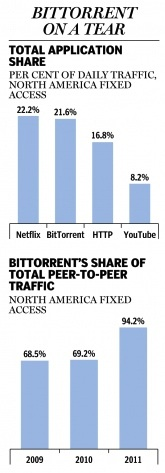
\includegraphics[width=0.5\textwidth]{p2p-stats1.jpg}
	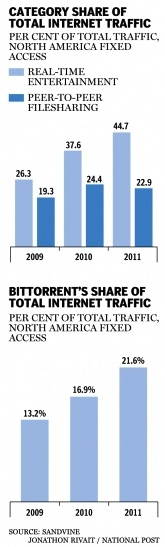
\includegraphics[width=0.5\textwidth]{p2p-stats2.jpg}\\
\end{column}
\end{columns}
\begin{flushright}
	{\tiny \url{http://business.financialpost.com/2011/07/01/bittorrent-turns-ten}}
\end{flushright}
\end{frame}

\begin{frame}{Legal (!) applications}
	
\BIL
\item Music, video and the like
	\BI
	\item BitTorrent Inc
	\item SubPop Records
	\item Norwegian Broadcasting Corporation
	\EI
\item Software
	\BI
	\item Linux distributions
	\item Blizzard: Diablo III, StarCraft II, World of Warcraft (game updates)
	\EI
\item Web services
\BI
\item Amazon S3 equipped with built-in BitTorrent support
\item Facebook, Twitter use BitTorrent to distribute updates to their servers
\EI
\EIL
\end{frame}

\begin{frame}{BitTorrent architecture}
	
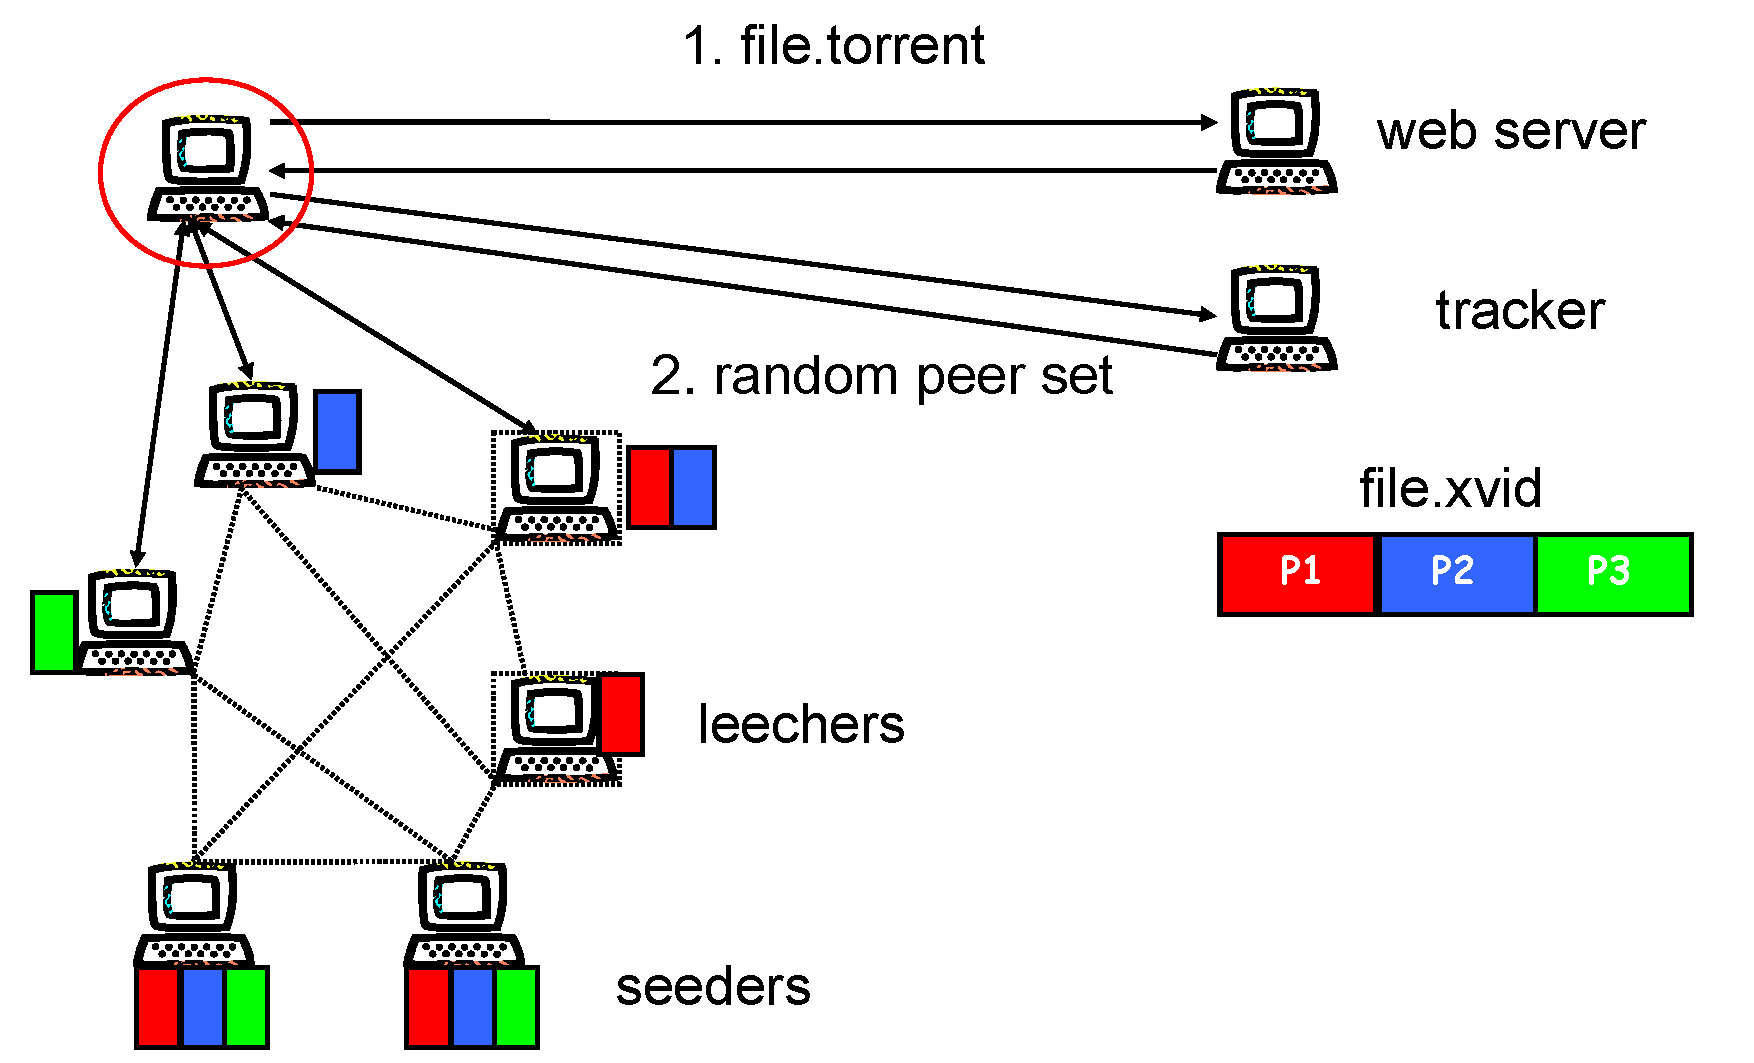
\includegraphics[width=\textwidth]{bt-arch}	
	
\end{frame}






\begin{frame}{Torrent file}
A torrent file is a \textit{bencoded} dictionary with the following keys:
\BI
\item \texttt{announce} -- the URL of the tracker
\item \texttt{name} -- suggested file/directory name
\item \texttt{piece length} -- number of bytes per piece (commonly $256$KB)
\item \texttt{pieces} -- a concatenation of each piece's SHA-1 hash. 
\item Exactly one of \texttt{length} or \texttt{files}:
	\BI
	\item \texttt{length} -- size of the file (in bytes)
	\item \texttt{files} -- a list of files with the following keys:
		\BI
		\item \texttt{path} - pathname of the file
		\item \texttt{length} - size of the file (in bytes)
		\EI
	\EI
\EI
\end{frame}

\begin{frame}{BitTorrent architecture}

\begin{columns}
\begin{column}{0.60\textwidth}
\BIL
\item \alert{Peer Selection}
	\BI
	\item “Which peers to upload to”
	\item Efficiency criteria:
		\BI
		\item Maximize service capacity
		\item Foster reciprocation and prevent free riders
		\EI
	\EI
\item \alert{Piece selection}
	\BI
	\item “Which pieces to download from selected peer”
	\item Should guarantee \textit{piece diversity}
		\BI
		\item Always find an interesting piece in selected peer
		\item Do not bias peer selection
		\EI
	\EI
\EIL
\end{column}	
\begin{column}{0.38\textwidth}
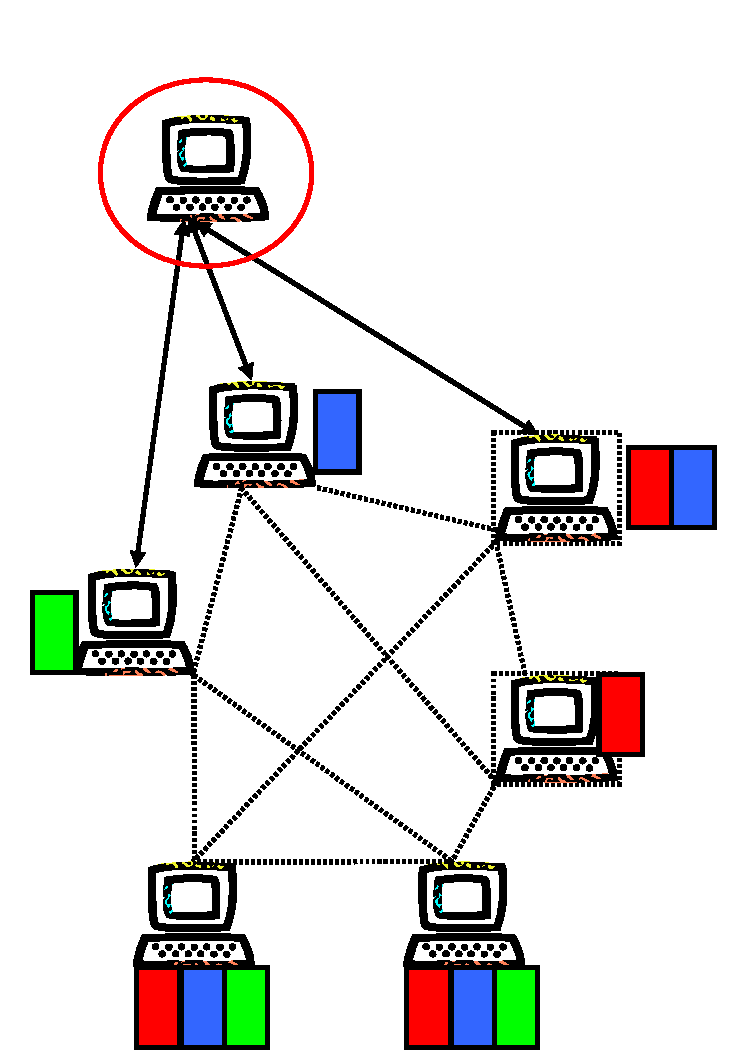
\includegraphics[width=\textwidth]{bt-arch2}	
\end{column}
\end{columns}
\end{frame}


\begin{frame}{Piece selection}
\BIL
\item The order in which pieces are selected by peers is critical
\item A bad algorithm could create a situation where all peers have all pieces that are currently
 available and none of the missing ones
\item If the original seed disappears, the download cannot be completed!
\EIL
\end{frame}

\begin{frame}{Policies}
	
\BIL
\item \alert{Strict Priority}
\BI
\item A piece is broken into sub-pieces (typically 16KB in size)
\item Policy: \textit{Until a piece is assembled, only download sub-pieces for that piece from the same source}
\item This policy lets complete pieces assemble quickly
\EI
\item \alert{Rarest first}
\BI
\item Policy: \textit{Determine the pieces that are most rare among your peers and download those first}
\item This ensures that the most common pieces are left till the end to download
\item Rarest first also ensures that a large variety of pieces are downloaded from the seed	
\EI
\EIL

\end{frame}

\begin{frame}{Policies}

\BIL
\item \alert{Random first piece}
\BI
\item Initially, a peer has nothing to trade
\item Important to get a complete piece ASAP
\item Rare pieces are typically available at fewer peers, so downloading a rare piece initially is not a good idea
\item Policy: \textit{Select a random piece of the file and download it}
\EI
\item \alert{Endgame mode}
\BI
\item Policy: \emph{When all the sub-pieces that a peer doesn't have are actively being requested, these are requested from \textbf{every} peer}
\item When the sub-piece arrives, the replicated requests are canceled
\item This ensures that a download doesn't get prevented from completion due to a single peer with a slow transfer rate
\item Some bandwidth is wasted; in practice, not too much
\EI
\EIL
\end{frame}

%-------------------------------------------------------------------------
\begin{frame}{Peer selection}

\structure{Choking}\\
\BIL	
\item Choking is a temporary refusal to upload; download occurs as normal
\item One of BitTorrent’s most powerful idea
\item It ensures that nodes cooperate and eliminates(?) the free-ride problem
\item When a node is unchoked, upload restart
\item Connection is kept open to reduce setup costs
\item Based on \alert{game-theoretic tit-for-tat strategy in repeated games}
\EIL

\end{frame}

%-------------------------------------------------------------------------
\begin{frame}{Prisoner's Dilemma}

Two men are arrested, but the police do not possess enough information 
for a conviction. Following the separation of the two men, the police offer 
both a similar deal:
	
\begin{table}
\begin{tabular}{|l||c|c|}
\hline
  & Prisoner $B$ & Prisoner $B$ \\
  & stays silent & confesses \\
\hline\hline
Prisoner $A$ stays silent & Both serve 1 months & $A$ serves 1 year \\
                        &                     & $B$ goes free \\
\hline
Prisoner $A$ confesses & $B$ serves 1 year & Both serve 3 months \\
                        & $A$ goes free &  \\
\hline
\end{tabular}
\end{table}
	
\end{frame}

%-------------------------------------------------------------------------
\begin{frame}{Prisoner's Dilemma}

\begin{block}{Single-iteration game}
\BIL
\item What is the best strategy?
\pause
\item “Confessing” is a dominant strategy
\BI
\item If the other prisoner confesses, the best move is to confess
\item If the other prisoner stay silent, the best move is to confess
\EI
\EIL
\end{block}

\pause
\begin{block}{What about iterated games?}
\pause
\BIL
\item Robert Axelrod's “The evolution of cooperation”
\item Tournament of computer programs playing PD
\item The winner: Tit-for-tat, Anatol Rapoport
\EIL
\end{block}

\end{frame}

%-------------------------------------------------------------------------
\begin{frame}{Prisoner's Dilemma}

\begin{block}{Tit-for-tat}
\BI
\item Be nice at the beginning
\item Do onto others as they do onto you: 
\item If the other prisoner confesses, you must retaliate back
\item Have a recovery mechanism to ensure eventual cooperation
\EI
\end{block}

\bigskip
How to translate this in BitTorrent?

\end{frame}

%-------------------------------------------------------------------------
\begin{frame}{Choking/unchoking}
	
\structure{Goal}: have several bidirectional connections running continuously\\
\BIL
\item Upload to peers who have uploaded to you recently
\BI
\item “Do onto others as they do onto you”
\EI
\item Unused connections are uploaded to on a trial basis to see if better transfer rates could be found using them
\BI
\item “Be nice at the beginning”
\item “Have a recovery mechanism to ensure eventual cooperation”	
\EI
\EIL
	
\end{frame}

%-------------------------------------------------------------------------
\begin{frame}{Choking/unchoking specifics}

\BIL
\item A peer always unchokes a fixed number of its peers (default: $4$)
\item Decision to choke/unchoke done based on current download rates, averaged over the last $20$s
\item Evaluation on who to choke/unchoke is performed every $10$s
	\BI
	\item Prevents wasting of resources by rapidly choking/unchoking peers
	\item Enough for TCP to ramp up transfers to their full capacity
	\EI
\item Which peer is the optimistic unchoke is rotated every $30$s
	\BI
	\item Used to discover if a currently choked peer would be better
	\EI
\EIL
\end{frame}

%-------------------------------------------------------------------------
\begin{frame}{Additional details}
	
\structure{Anti-snubbing}:\\
\BIL
\item A peer is said to be \alert{snubbed} if each of its peers chokes it
\item To handle this, snubbed peer stops uploading to its peers
\item Optimistic unchoking done more often
\BI
\item Hope is that will discover a new peer that will upload to us
\EI
\EIL

\structure{Seeding}:
\BIL
\item Once download is complete, a peer has no download rates to use for comparison nor has any need to use them
\item The question is, which nodes to upload to?
\item Policy: Upload to those with the best upload rate.
\BI
\item This ensures that pieces get replicated faster
\EI
\EIL

\end{frame}

\begin{frame}{Improvements over the tracker bottleneck}

\BIL
\item \alert{Trackerless BitTorrent} (i.e., w/o a centralized tracker):
\BI
\item Based on variants of Kademlia DHT
\item Tracker run by a normal end-host
\item Vuze DHT vs Mainline DHT
\EI
\item \alert{Peer Exchange (PEX)}:
\BI
\item Each peer directly update other peers as to which peers are currently in the swarm
\item Epidemic sampling!
\item Three incompatible version of PEX (Vuze, BitComet, Mainline)
\EI
\item \alert{Multitracking}
\BI
\item Multiple trackers in the torrent file
\EI
\EIL

\end{frame}

%-------------------------------------------------------------------------
\begin{frame}{Five months in a torrent's lifetime}
	
	
\BI
\item Analysis of a tracker log
\item 1.77GB Linux Redhat 9 distribution
\item Five months - April-August 2003
\item 180.000 downloads
\EI	

\bigskip
\begin{Bib}
{\scriptsize
\bibentry{fivemonths} 
}
\end{Bib}	

	
\end{frame}


%-------------------------------------------------------------------------
\begin{frame}{Network: Number of active peers over time}
	
\begin{figure}	
	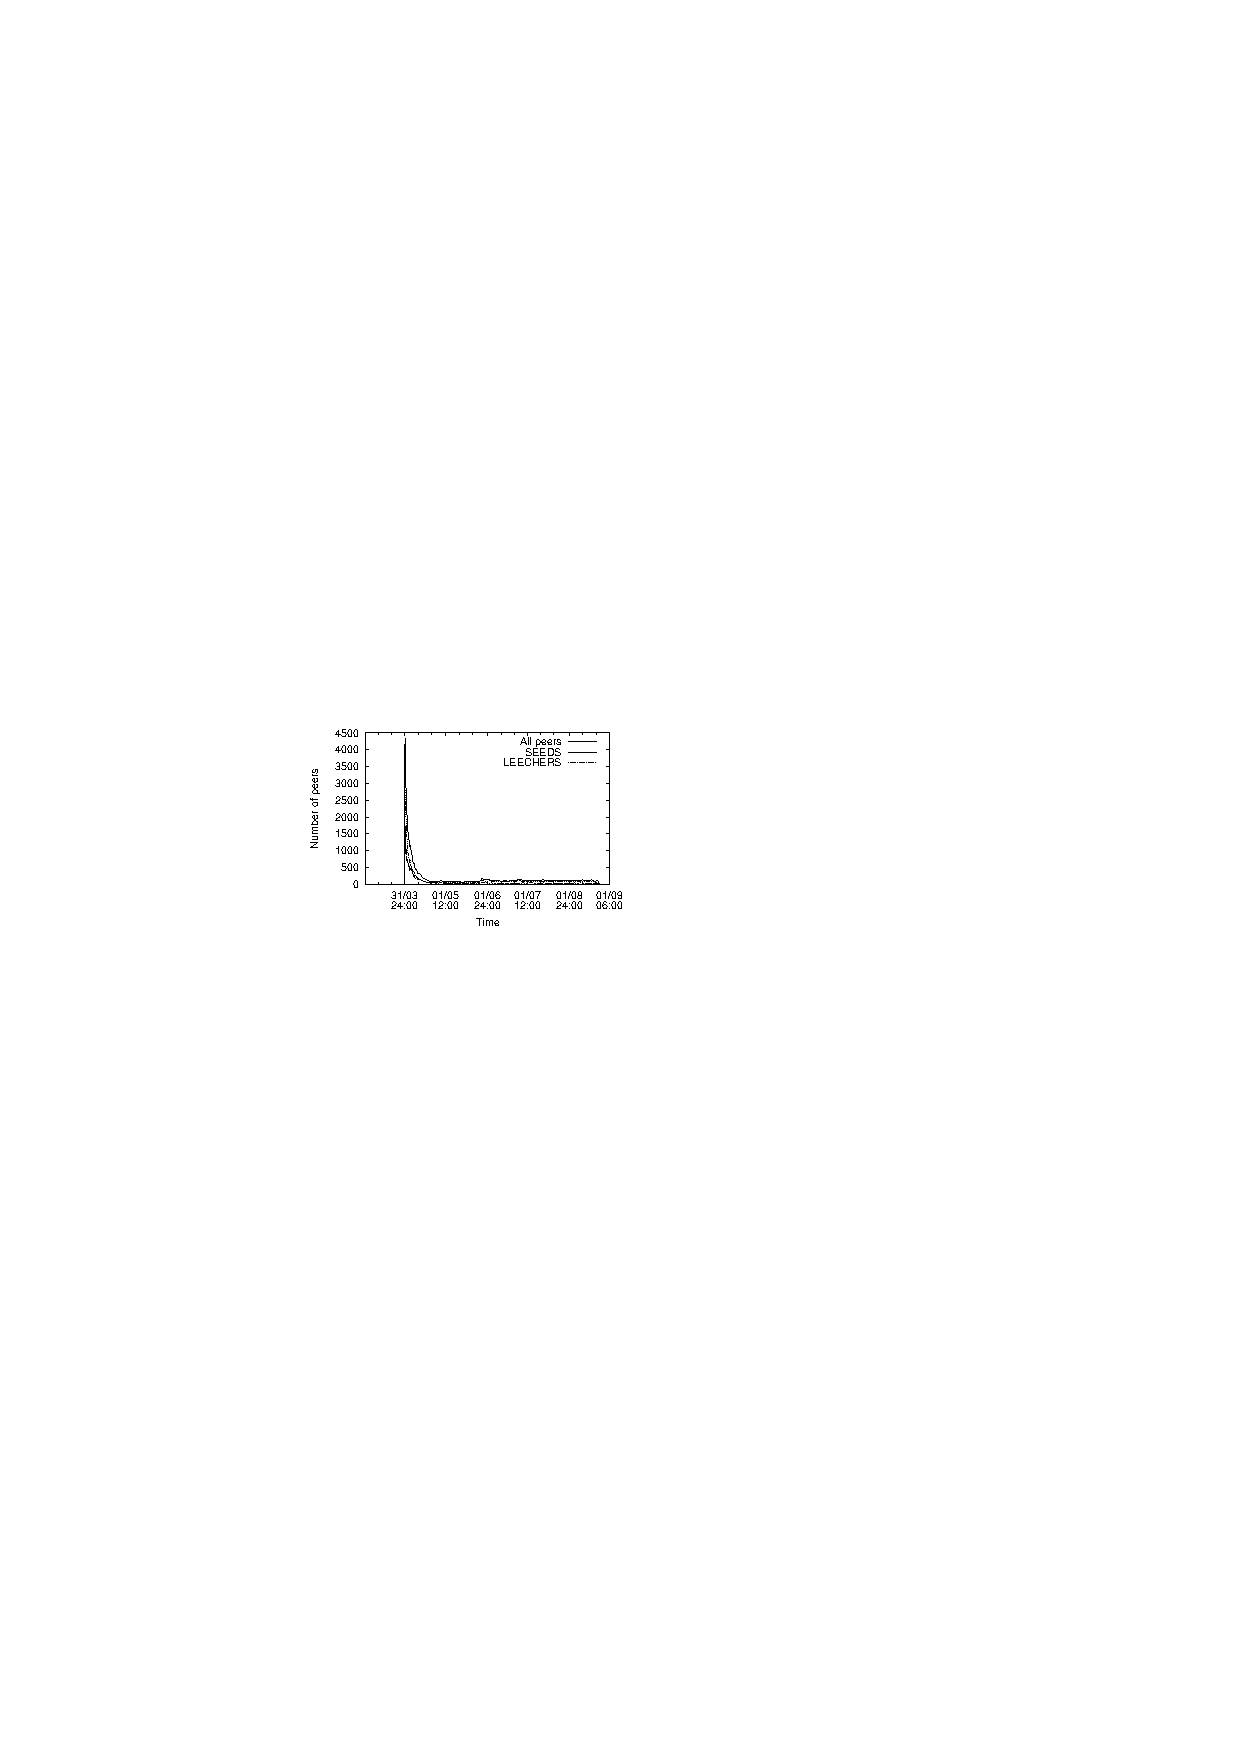
\includegraphics[width=0.85\textwidth]{bt-fig1}
	\caption{Complete trace}
\end{figure}	
	
\end{frame}

%-------------------------------------------------------------------------
\begin{frame}{Network: Number of active peers over time}
	
\begin{figure}	
	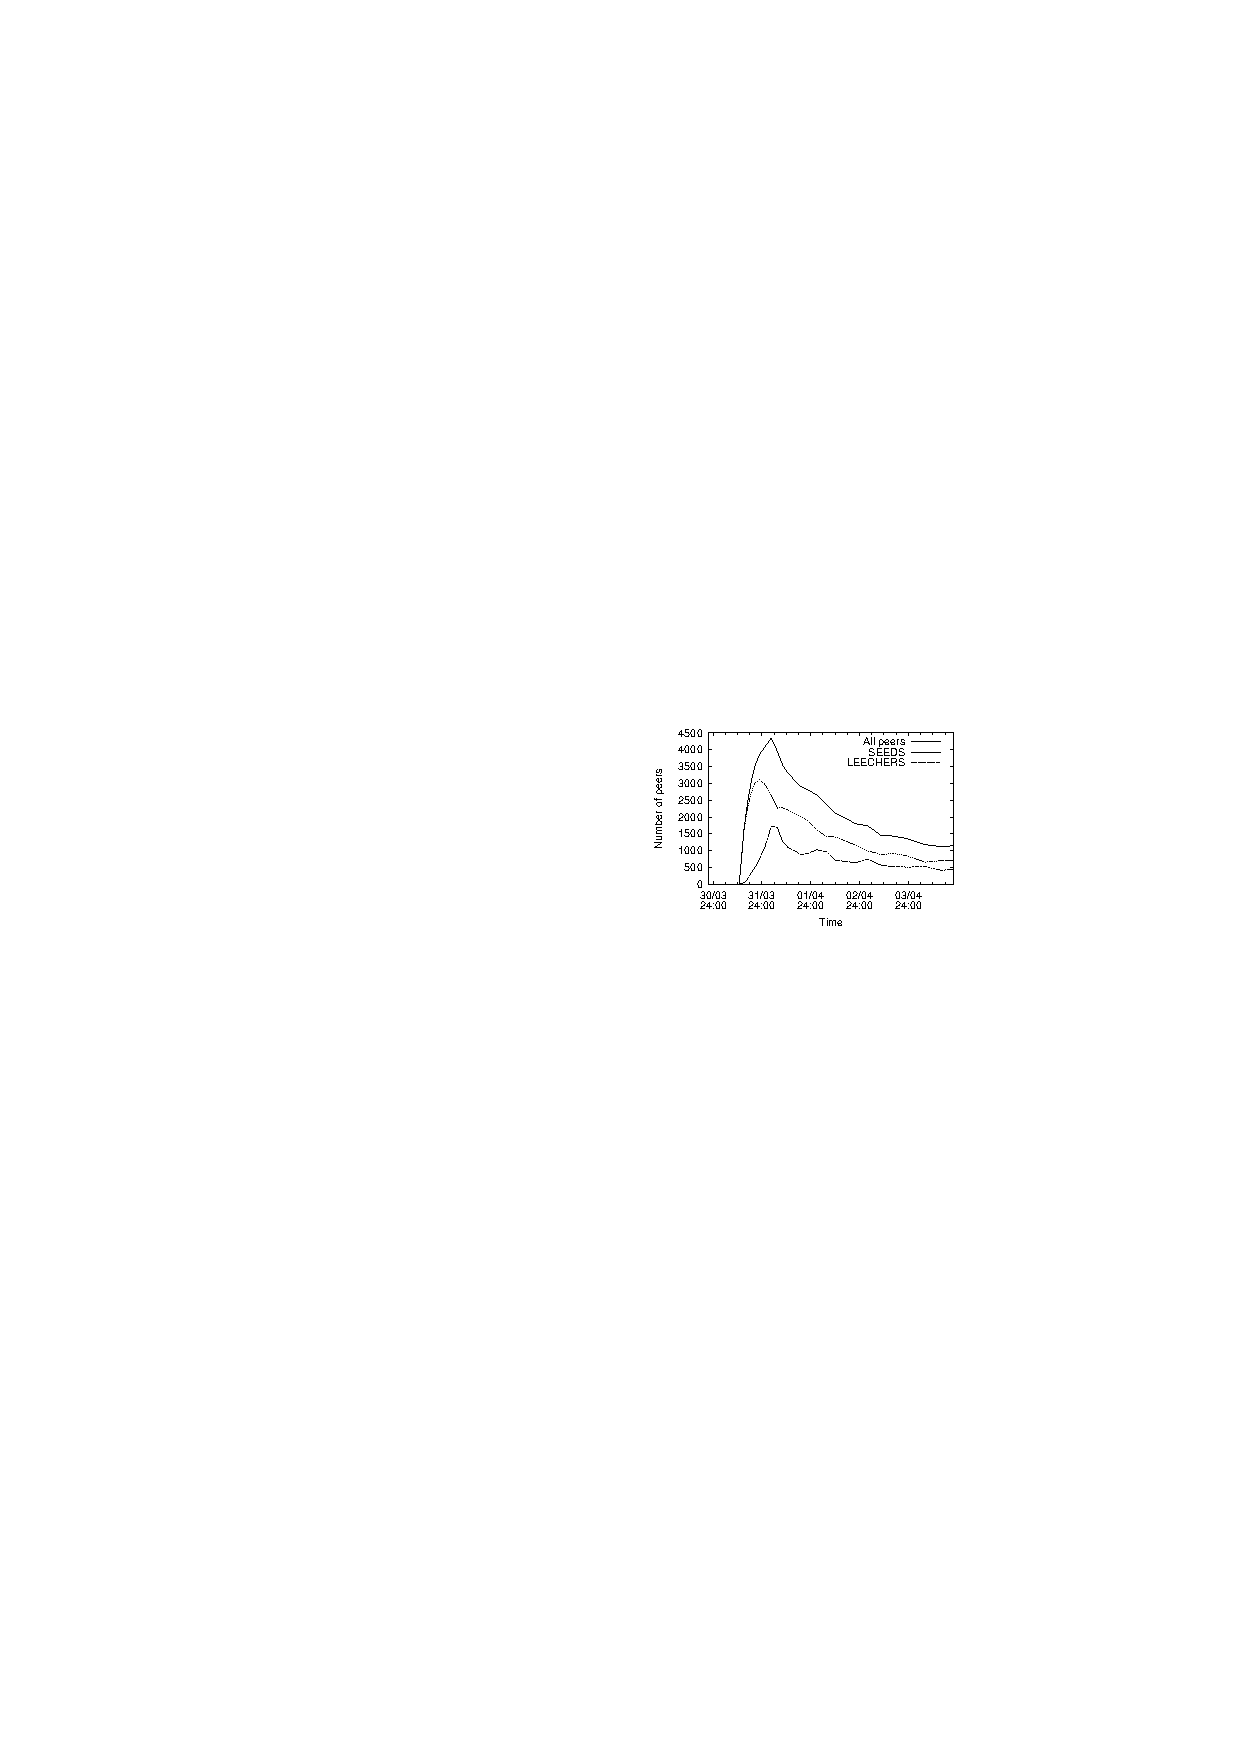
\includegraphics[width=0.79\textwidth]{bt-fig2}
	\caption{First five days}
\end{figure}	
	
\end{frame}

%-------------------------------------------------------------------------
\begin{frame}{Network: Proportion of seeders and leechers}
	
\begin{figure}	
	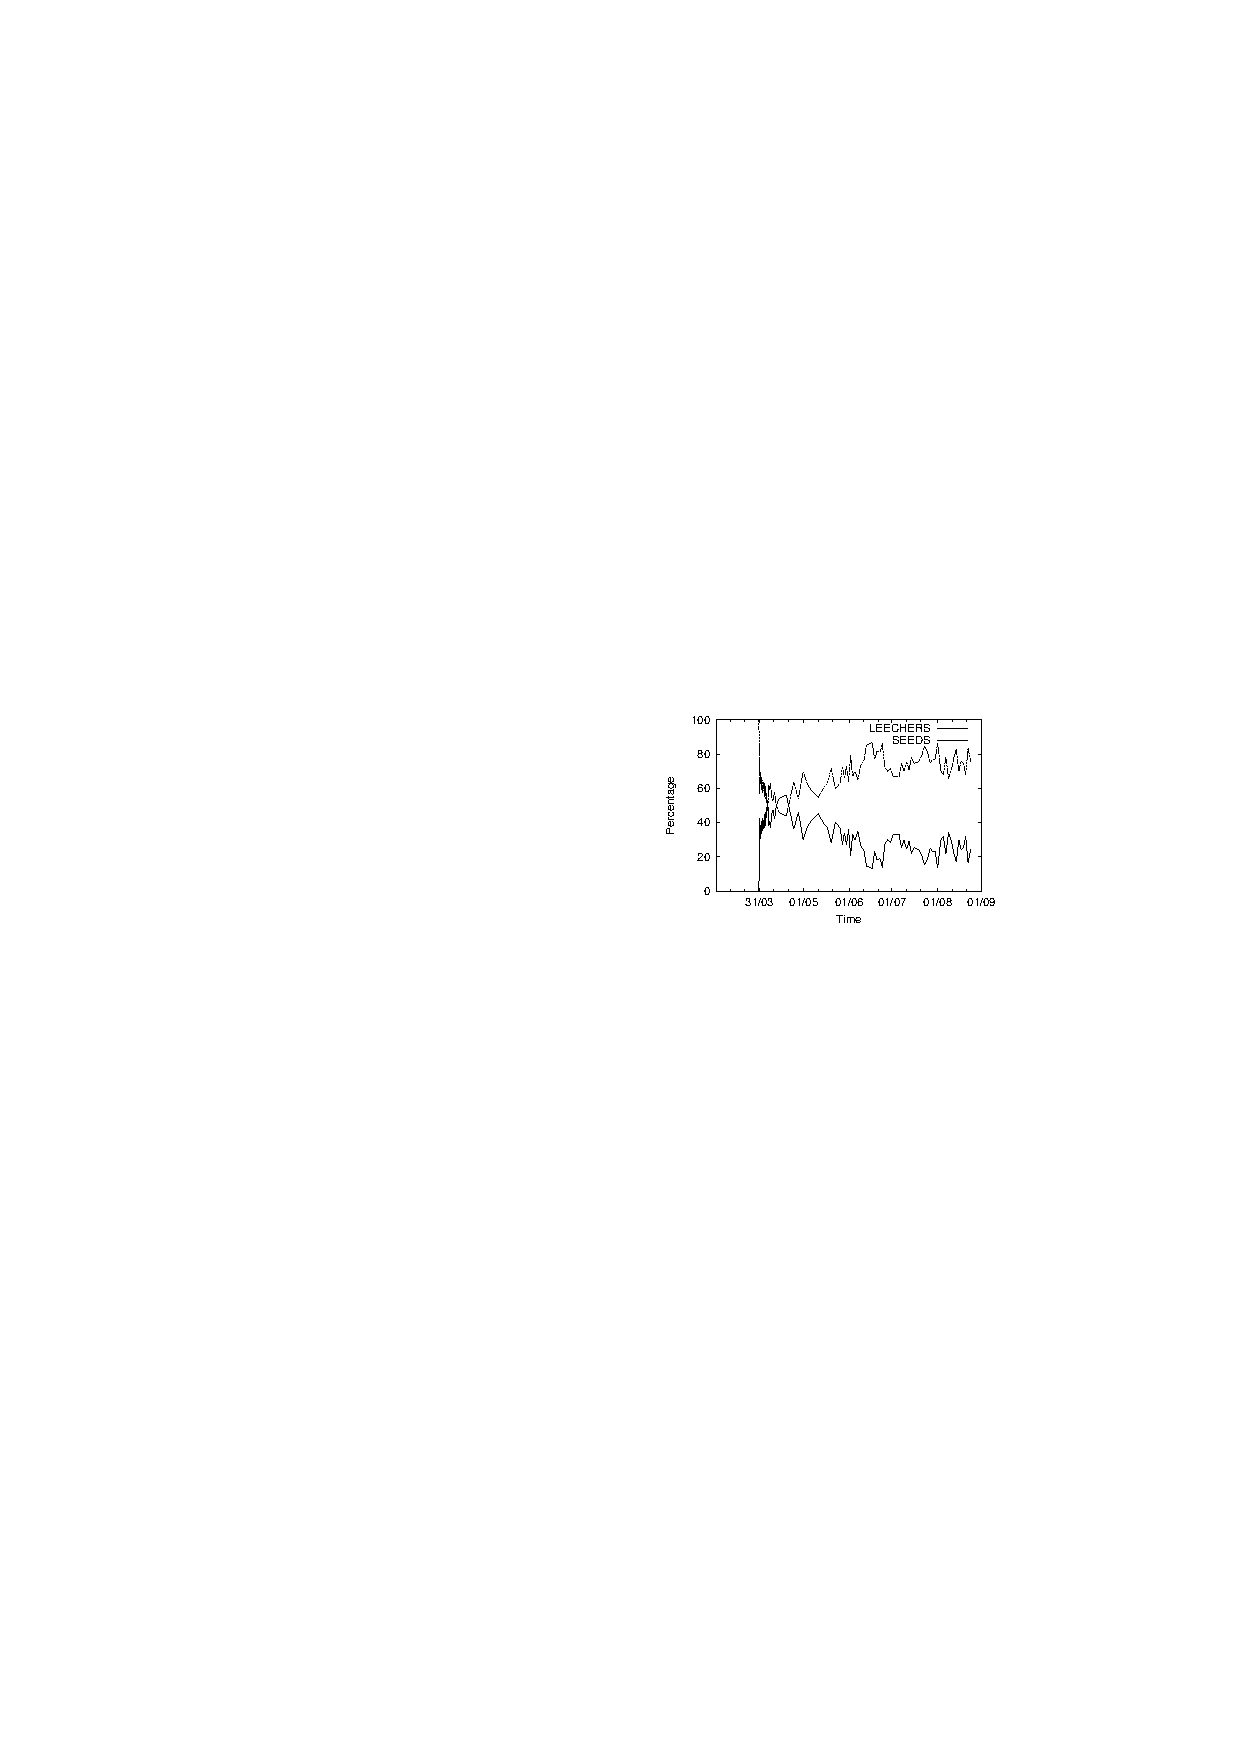
\includegraphics[width=0.79\textwidth]{bt-fig6}
	\caption{Complete trace}
\end{figure}	
	
\end{frame}


%-------------------------------------------------------------------------
\begin{frame}{Client: Cumulative download and upload evolution}
	
\begin{figure}	
	\includegraphics[width=0.79\textwidth]{bt-fig3}
	\caption{Complete torrent}
\end{figure}	
	
\end{frame}

%-------------------------------------------------------------------------
\begin{frame}{Client: Cumulative download and upload evolution}
	
\begin{figure}	
	\includegraphics[width=0.79\textwidth]{bt-fig4}
	\caption{First ten minutes}
\end{figure}	
	
\end{frame}

%-------------------------------------------------------------------------
\begin{frame}{Client: Number of connected peers}

\begin{figure}	
	\includegraphics[width=0.79\textwidth]{bt-fig5}
	\caption{Around 14 hours}
\end{figure}	
	
\end{frame}

%-------------------------------------------------------------------------
\begin{frame}[shrink]{Cheating BitTorrent}

\BIL
\item Tit-for-tat strategy has been designed to foster reciprocation
\item Nevertheless, its incentives are not robust to strategic clients
\item Two examples:
	\BI
	\item \alert{BitTyrant}
		\BI
		\item a strategic client that tries to improve download/upload rate
		\EI
	\item \alert{BitThief}
		\BI
		\item a client that never uploads anything
		\EI
	\EI
\EIL

\begin{Bib}
{\scriptsize
\BI
\item	\bibentry{bittyrant}
\item 	\bibentry{bitthief}
\EI
}
\end{Bib}

\end{frame}

%-------------------------------------------------------------------------
\begin{frame}{BitTyrant}

\structure{How to improve performance?}
\BI
\item Maximize reciprocation bandwidth per connection
\item Maximize number of reciprocating peers
\item Deviate from equal split
\EI

\smallskip
\begin{block}{Unchoking algorithm}
\BI
\item $d_p$: download rate of connection $p$
\item $u_p$: upload rate of connection $p$
\item Each round, rank peers by the ratio $u_p/d_p$ and unchoke the first
$k$ such that the upload capacity is reached:
\[
\sum_{i=1}^k u_i \leq \mathit{cap}
\]
\EI
\end{block}
\end{frame}

%-------------------------------------------------------------------------
\begin{frame}{BitTyrant}

\includegraphics[width=\textwidth]{bittyrant1}

\end{frame}

%-------------------------------------------------------------------------
\begin{frame}{BitThief}

\begin{columns}
\begin{column}{0.44\textwidth}
\structure{Download only: benefits}
\BI
\item no copyright issues (only contributors are sued)
\item conserve resources
\item spoil the community
\EI

\bigskip
\begin{figure}
\includegraphics[width=0.8\textwidth]{bitthief1}
\end{figure}
\end{column}
\begin{column}{0.56\textwidth}
\structure{Gains from optimistic unchoking}:
\BI
\item Ask for as many clients as possible
	\BI
	\item Increment tracker polling
	\item Decentralized tracking, PEX
	\EI
\item Connect to all available clients
	\BI
	\item higher chance of being unchoked
	\EI
\item Always pretend to be a newcomer
	\BI
	\item Advertise no pieces
	\item Download whatever available
	\item Most clients are nice
	\EI
\EI

\structure{Gains from free sharing of seeders}:
\BI
\item Seeders select peers in two ways:
	\BI
	\item highest bandwidth
	\item round robin
	\EI
\item BitThief report high upload rate
\EI

\end{column}
\end{columns}

\end{frame}

%-------------------------------------------------------------------------
\begin{frame}{BitThief}

\begin{columns}
\begin{column}{0.40\textwidth}
\begin{figure}
	\includegraphics[width=\textwidth]{bitthief2}
	\caption{With seeders}
\end{figure}
\end{column}
\begin{column}{0.40\textwidth}
\begin{figure}
	\includegraphics[width=\textwidth]{bitthief3}
	\caption{Without seeders}
\end{figure}
\end{column}
\end{columns}

\begin{figure}
	\includegraphics[width=0.4\textwidth]{bitthief4}
\end{figure}

\end{frame}

%-------------------------------------------------------------------------
\begin{frame}{Tribler}



\begin{columns}
\begin{column}{0.45\textwidth}
\structure{Problem}:\\
\BI
\item Most users have different upload/download speeds
\item Tit-for-tat may restrict the download speed
\item Solution: let your friends help you for free
\EI
\end{column}
\begin{column}{0.55\textwidth}
\begin{figure}
	\includegraphics[width=\textwidth]{tribler2}
\end{figure}
\end{column}
\end{columns}

\smallskip
\begin{Bib}
{\scriptsize
\bibentry{tribler}
}

\end{Bib}


\end{frame}

%-------------------------------------------------------------------------
\begin{frame}{Tribler}

\begin{figure}
	\includegraphics[width=1.0\textwidth]{tribler1}
\end{figure}

\end{frame}



%-------------------------------------------------------------------------


\begin{RMFrame}

\BI
\item \bibentry{p2psurvey}
\EI

\end{RMFrame}





\end{document}